%==============TODOS====================
% Convolution strukturiert in modulations einheit packen.
% Evtl kleine animation in python machen. Evtl zusammenhang zu FIR filter expliziter.
% Fourier einheit ausarbeiten, Physical modelling Einheit ausarbeiten.
% Modulation: FM parametriesierung recherchieren.
% Notations konsitenz ueberpruefen v.a. eckige vs. runde klammern f discrete signale.

%Dokumentklasse
\documentclass[a4paper,11pt]{scrreprt}
% scrbook
% \documentclass[a4paper,11pt]{scrbook}

\usepackage[left= 3.5cm,right = 3cm, bottom = 3.5 cm, top = 3 cm]{geometry}
\usepackage[onehalfspacing]{setspace}
% ============= Packages =============

% \usepackage{silence}
% \WarningFilter[pdftoc]{hyperref}{Token not allowed in a PDF string}

% Standard Packages
\usepackage[utf8]{inputenc}
\usepackage[english]{babel} % english
\usepackage[T1]{fontenc}
\usepackage{graphicx}
\usepackage{graphicx, subfigure}
\graphicspath{{img/}} %setze pfad fuer Bilder
% \usepackage{fancyhdr}
\usepackage{lmodern}
\usepackage{color}
\usepackage{transparent}
% Citation style
\usepackage[comma,authoryear]{natbib}
% zusätzliche Schriftzeichen der American Mathematical Society
\usepackage{amsfonts}
\usepackage{mathtools}
% BlockDiagram Drawing Package
\usepackage{tikz}
\usetikzlibrary{positioning}
\usepackage{pgfplots}
\pgfplotsset{compat=1.10}
\usepackage{textcomp}
%Package for using the [H] option on graphics to force them into place
\usepackage{float}
%iPython packages:
\usepackage{adjustbox} % Used to constrain images to a maximum size
\usepackage{enumerate} % Needed for markdown enumerations to work
% \usepackage{geometry} % Used to adjust the document margins
\usepackage{amsmath} % Equations
\usepackage{amssymb} % Equations
% \usepackage{mathrsfs}
\usepackage[mathletters]{ucs} % Extended unicode (utf-8) support
% \usepackage[utf8x]{inputenc} % Allow utf-8 characters in the tex document
\usepackage{fancyvrb} % verbatim replacement that allows latex
\usepackage{grffile} % extends the file name processing of package graphics
                         % to support a larger range
    % The hyperref package gives us a pdf with properly built
    % internal navigation ('pdf bookmarks' for the table of contents,
    % internal cross-reference links, web links for URLs, etc.)
% \usepackage{hyperref}
\usepackage{longtable} % longtable support required by pandoc >1.10
\usepackage{scrhack}
\usepackage{framed}

\usepackage{atbegshi}% http://ctan.org/pkg/atbegshi

\usepackage{listings}
\usepackage{todonotes}
\usepackage{courier}

% Dokumentinformationen
\usepackage[
	pdftitle={dsp course},
	pdfsubject={},
	pdfauthor={Patrik Lechner},
	pdfkeywords={}
	pdftex=true,
	colorlinks=true,
 	breaklinks=true,
	citecolor=black,
	linkcolor=blue,
	menucolor=black,
	urlcolor=blue
]{hyperref}

\hypersetup{
    % bookmarks=true,         % show bookmarks bar?
    unicode=false,          % non-Latin characters in Acrobat’s bookmarks
    pdftoolbar=true,        % show Acrobat’s toolbar?
    pdfmenubar=true,        % show Acrobat’s menu?
    pdffitwindow=false,     % window fit to page when opened
    pdfstartview={FitH},    % fits the width of the page to the window
    pdftitle={EPRO/IAS Scriptum},    % title
    pdfauthor={Patrik Lechner},     % author
    pdfsubject={EPRO/IAS},   % subject of the document
    pdfcreator={Patrik Lechner},   % creator of the document
    pdfproducer={Patrik Lechner}, % producer of the document
    pdfkeywords={dsp} {pure data} {audio}, % list of keywords
    pdfnewwindow=true,      % links in new window
    colorlinks=true,       % false: boxed links; true: colored links
    linkcolor=gray,          % color of internal links (change box color with linkbordercolor)
    citecolor=black,        % color of links to bibliography
    filecolor=black,      % color of file links
    urlcolor=blue           % color of external links
}





% embedding of audio/video files etc.
% \usepackage{attachfile}
% \usepackage{movie15}
% \usepackage{media9}
% \usepackage{menukeys}


% =============== BlockDiagram Drawing Config
\usetikzlibrary{shapes,arrows}
  \usetikzlibrary{mindmap,trees, backgrounds}

% Definition of blocks:
\tikzset{%
  block/.style    = {draw, thick, rectangle, minimum height = 3em,
    minimum width = 3em},
  sum/.style      = {draw, circle, node distance = 2cm}, % Adder
  input/.style    = {coordinate}, % Input
  output/.style   = {coordinate}, % Output
  mult/.style	  = {draw, isosceles triangle, minimum height=1cm, minimum width =1cm}
}
% mult/.style	  = {isosceles triangle, sharp corners, anchor=center, xshift=-4mm, minimum height=1.5cm, minimum width =0.05cm}
%isosceles triangle, fill=gray!25, minimum width=1.5cm

% Defining string as labels of certain blocks.
\newcommand{\suma}{\Large$+$}
\newcommand{\inte}{$\displaystyle \int$}
\newcommand{\derv}{\huge$\frac{d}{dt}$}
\newcommand{\conv}{\huge$\ast$}

% ============================================

% -- Settings für Code abbildungen
% \usepackage{listings}

% \definecolor{dkgreen}{rgb}{0,0.6,0}
% \definecolor{gray}{rgb}{0.5,0.5,0.5}
% \definecolor{mauve}{rgb}{0.58,0,0.82}

% \lstset{frame=tb,
%   language=Java,
%   aboveskip=3mm,
%   belowskip=3mm,
%   showstringspaces=false,
%   columns=flexible,
%   basicstyle={\small\ttfamily},
%   numbers=none,
%   numberstyle=\tiny\color{gray},
%   keywordstyle=\color{blue},
%   commentstyle=\color{dkgreen},
%   stringstyle=\color{mauve},
%   breaklines=true,
%   breakatwhitespace=true
%   tabsize=3
% }




% Setze arial font
% \renewcommand*{\familydefault}{\sfdefault}

% FH-grünBlau
\definecolor{FH}{rgb}{0.10, 0.57, 0.68}



% nicht einrücken nach Absatz
\setlength{\parindent}{0pt}


% ============= Kopf- und Fußzeile =============
% \pagestyle{fancy}
%
% \lhead{}
% \chead{}
% \rhead{\slshape \leftmark}
%%
% \lfoot{}
% \cfoot{}
% \rfoot{\thepage}
%%
% \renewcommand{\headrulewidth}{0.4pt}
% \renewcommand{\footrulewidth}{0pt}

% ============= Remove first Page======

\AtBeginDocument{\AtBeginShipoutNext{\AtBeginShipoutDiscard}}

%======================================


\usepackage[framemethod=tikz]{mdframed}
\newtheorem{question}{Question}
\mdfdefinestyle{que}{
  linecolor=cyan,
  backgroundcolor=cyan!20,
}
\surroundwithmdframed[style=que]{question}

\newtheorem{answer}{Answer}
\mdfdefinestyle{ans}{
  linecolor=cyan,
  backgroundcolor=yellow!20
  % , rotatebox
}
\surroundwithmdframed[style=ans]{answer}

\usepackage{environ}
\NewEnviron{Answer}
{%
\noindent
\rotatebox[origin=c]{180}{%
\noindent
\begin{minipage}[t]{\linewidth}
\begin{answer}
\BODY
\end{answer}%
\end{minipage}%
}%
}%



% ============= Package Einstellungen & Sonstiges =============

%COMMENT
\newcommand{\comm}[1]{\Large{\color{red}{#1}}\normalsize{}}


%Besondere Trennungen
\hyphenation{De-zi-mal-tren-nung St-rei-fen-licht-scan-nern}

%römische Aufzählungen mit \RM{Zahl}
\newcommand{\RM}[1]{\MakeUppercase{\romannumeral #1}}

\newcommand{\pd}[1]{\texttt{[{#1}]}}
\newcommand{\link}[2]{\href{#1}{#2}\footnote{#1}}
\usepackage{mdframed}

\newcommand{\bgInfo}[1]{\begin{mdframed}[backgroundcolor=black!10,rightline=false,leftline=false] #1 \end{mdframed}}

\newcommand{\video}[1]{
\begin{framed}
\textbf{Video Analogies}\\
 #1 \end{framed}}


\newcommand{\important}[1]{\begin{framed} #1 \end{framed}}



\definecolor{mygreen}{RGB}{28,172,0} % color values Red, Green, Blue
\definecolor{mylilas}{RGB}{170,55,241}



% ============= Dokumentbeginn =============

\begin{document}


% ==========Matlab code formatting================
\lstset{language=Matlab,%
    %basicstyle=\color{red},
    basicstyle=\footnotesize\ttfamily,
    breaklines=true,%
    morekeywords={matlab2tikz},
    keywordstyle=\color{blue},%
    morekeywords=[2]{1}, keywordstyle=[2]{\color{black}},
    identifierstyle=\color{black},%
    stringstyle=\color{mylilas},
    commentstyle=\color{mygreen},%
    showstringspaces=false,%without this there will be a symbol in the places where there is a space
    % numbers=left,%
    % numberstyle={\tiny \color{black}},% size of the numbers
    % numbersep=9pt, % this defines how far the numbers are from the text
    emph=[1]{for,end,break},emphstyle=[1]\color{red}, %some words to emphasise
    %emph=[2]{word1,word2}, emphstyle=[2]{style},
}
% ================================================




%!TEX root = main.tex

\pagestyle{empty}
\begin{center}
\begin{tabular}{p{\textwidth}}


\begin{center}
\includegraphics[scale=0.7]{img/FHlogo.jpg}
\end{center}

\\

\begin{center}
\Huge{{\color{FH}{\fontsize{24}{48} \selectfont Signal Processing\\}}}
\end{center}

\\

\\

\begin{center}
Bachelor Studiengang Medientechnik\\
Fachhochschule St.Pölten
\end{center}

\\
\begin{center}
Patrik Lechner
\end{center}

\\

\begin{center}
\large{Wien, \today}
\end{center}


\end{tabular}
\end{center}

% \part im Inhaltsverzeichnis nicht nummerieren
\makeatletter
\let\partbackup\l@part
\renewcommand*\l@part[2]{\partbackup{#1}{}}

% Chapter number reset at new part.
% \@addtoreset{chapter}{part}

%Seitennummerierung neu beginnen, Zahlen [arabic], röm.Zahlen [roman,Roman], Buchstaben [alph,Alph]
% \pagenumbering{Roman}

% \newpage
%
% \include{02_Erklaerung}
% \newpage
% \include{03_zusammenfassung}

\newpage
% \include{tester}
%!TEX root = main.tex

\pagestyle{empty}
\begin{center}
\begin{tabular}{p{\textwidth}}


\begin{center}
\includegraphics[scale=0.7]{img/FHlogo.jpg}
\end{center}

\\

\begin{center}
\Huge{{\color{FH}{\fontsize{24}{48} \selectfont Signal Processing\\}}}
\end{center}

\\

\\

\begin{center}
Bachelor Studiengang Medientechnik\\
Fachhochschule St.Pölten
\end{center}

\\
\begin{center}
Patrik Lechner
\end{center}

\\

\begin{center}
\large{Wien, \today}
\end{center}


\end{tabular}
\end{center}
%!TEX root = main.tex

\chapter{Introduction}
\label{introduction}

\begin{figure}[h!]
	\centering
	\includegraphics[width=\textwidth]{intro}
	\caption[cover]
	{Weird effects of digital signals in video. }
	\label{fig:weirdVideo}
\end{figure}
\clearpage

This section tries to make sure we are all on the same page. It goes through some mathematics notation and principles of digital audio.\\
If you rather want a video format revision of digital audio (I mean, it's \the\year, of course you want), I can recommend \href{https://www.youtube.com/watch?v=cIQ9IXSUzuM}{D/A and A/D | Digital Show and Tell (Monty Montgomery @ xiph.org) }\footnote{https://www.youtube.com/watch?v=cIQ9IXSUzuM}. Some of the points in the video go beyond what we are doing here and vice versa, so don't purely rely on the video though. \\
Ideally, if you throughly understood the introduction section, you should be able to go through the remaining chapters with tempo.\\

\section{About this document}
Please report any mistakes, errors etc to \href{mailto:ptrk.lechner@gmail.com}{ptrk.lechner@gmail.com}.\\

Some information in this document is relevant for understanding its contents but not relevant for the exam. For example in chapter \ref{chap:modulation} we will find a really complicated result of an equation. The point there is just that it's complicated. And it is shown how complicated, but this is nothing to be learned by heart. Importance is tried to be made clear using the following formats:\\

\bgInfo{
Text, figures, and equations with a gray background like this are background information that is not to be learned by heart.}

\video{
This document tries to explain digital signals. It does this by use of audio signals mainly. Sometimes video analogies are given. These are also not relevant for the exam.
}

\important{Very important things are framed.}

Internal links are gray. You can click them to jump to another point in this document, such as Equation \ref{eq:dft}.\\

External links are blue, these are mostly links on the web. The actual link is always available as a footnote as well. \link{https://www.youtube.com/watch?v=57PWqFowq-4}{Here is an example}

Max objects will always be in courier new and square brackets. Like this: \pd{metro}.\\


\subsection{Programming Languages}
This Document tries to give examples in different programming languages. \link{https://cycling74.com/}{Max/MSP 8}, \link{https://www.python.org/}{python} in the form of \link{https://jupyter.org/}{jupyter notebooks} and \link{https://www.khronos.org/opengl/wiki/Core\_Language\_(GLSL)}{GLSL} in the form of \link{https://shadertoy.com/}{shadertoy} links.

\subsubsection*{Max/MSP}
This document was originally written for \textit{pd-extended}, a free open source alternative to Max/MSP. It is now in the process of migrating everything to Max/MSPversion:\\
8.0.0.
The following additional libraries are used:
\begin{itemize}
	\item HISSTools Impulse Response Toolbox (HIRT) (mostly used for its improved spectrogram)
	\item cv.jit (Computer vision)
\end{itemize}
Additionally the following libraries are recommended:
\begin{itemize}
	\item Max ToolBox (Allowing for faster patching)
	\item zsa.descriptors (Audio Feature extraction and analysis)
	\item MuBu for Max (Advanced pattern recognition and audio analysis)
\end{itemize}

\subsubsection*{iPython}

This document is in the process of transporting most plots and examples to interactive Collab Notebooks \link{https://colab.research.google.com/notebooks/welcome.ipynb}{Collab Notebooks} where one can see how the plot is made using python and one can play around with the settings interactively. You can run these notebooks in the browser with a google account(recommended) or you can install jupyter notebook on your machine to run them locally. Here is the notebook for the introduction section: \link{https://colab.research.google.com/github/hrtlacek/dspCourse/blob/master/notebooks/00\_Introduction.ipynb}{click here}.

\begin{figure}[H]
	\centering
	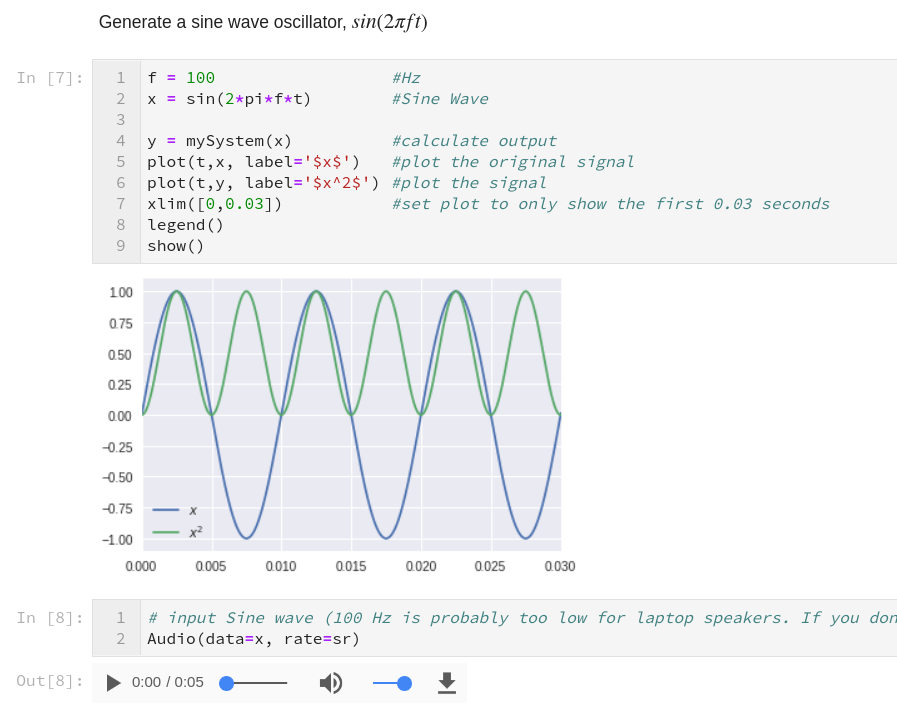
\includegraphics[width=\textwidth]{img/notenookExample.png}
	\caption[example of iPython notebook]
	{example of iPython notebook}
	\label{fig:ipython}
\end{figure}

\subsubsection*{GLSL}
\todo[inline]{unfinished}

\section{About plotting signals}

We will need to plot a lot of signals in order to understand them better. Most of the time, such a plot will look like figure \ref{fig:simpeSine}.

\begin{figure}[h!]
	\centering
	% This file was created with tikzplotlib v0.9.14.
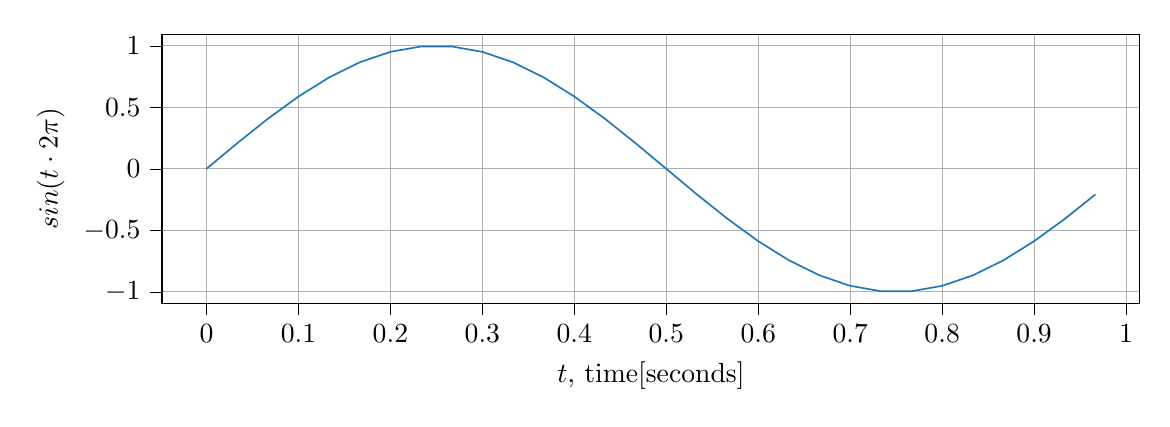
\begin{tikzpicture}

\definecolor{color0}{rgb}{0.12156862745098,0.466666666666667,0.705882352941177}

\begin{axis}[
height=5cm,
tick align=outside,
tick pos=left,
width=14cm,
x grid style={white!69.0196078431373!black},
xlabel={\(\displaystyle t\), time[seconds]},
xmajorgrids,
xmin=-0.0483333333333333, xmax=1.015,
xtick style={color=black},
y grid style={white!69.0196078431373!black},
ylabel={\(\displaystyle sin(t \cdot 2 \pi)\)},
ymajorgrids,
ymin=-1.0939740849051, ymax=1.0939740849051,
ytick style={color=black}
]
\addplot [semithick, color0]
table {%
0 0
0.0333333333333333 0.207911690817759
0.0666666666666667 0.4067366430758
0.1 0.587785252292473
0.133333333333333 0.743144825477394
0.166666666666667 0.866025403784439
0.2 0.951056516295154
0.233333333333333 0.994521895368273
0.266666666666667 0.994521895368273
0.3 0.951056516295154
0.333333333333333 0.866025403784439
0.366666666666667 0.743144825477394
0.4 0.587785252292473
0.433333333333333 0.4067366430758
0.466666666666667 0.207911690817759
0.5 1.22464679914735e-16
0.533333333333333 -0.207911690817759
0.566666666666667 -0.4067366430758
0.6 -0.587785252292473
0.633333333333333 -0.743144825477394
0.666666666666667 -0.866025403784438
0.7 -0.951056516295154
0.733333333333333 -0.994521895368273
0.766666666666667 -0.994521895368273
0.8 -0.951056516295154
0.833333333333333 -0.866025403784439
0.866666666666667 -0.743144825477394
0.9 -0.587785252292473
0.933333333333333 -0.4067366430758
0.966666666666667 -0.20791169081776
};
\end{axis}

\end{tikzpicture}

	% \includegraphics[width=11cm]{simpleSine}
	\caption[simple sine plot]
	{Sine wave, 1Hz, sampled at 30Hz sample rate}
	\label{fig:simpeSine}
\end{figure}

This plot looks nice but it has a problem. The sine wave is sampled at a sampling rate of 30 Hz, but we see a continuous line. This ``connection of the dots'' is created by plotting. It is kind of similar to what our \textit{digital-to-analog-converter} does. It somehow\footnote{linear interpolation in case of the plot} interpolates the values we have. \\
This can be misleading, so we should actually plot something more like figure \ref{fig:scatter}. Often we can see plots that look like figure \ref{fig:stem} as well when a signal is analyzed.

\begin{figure}[H]
	\centering
	% This file was created with tikzplotlib v0.9.14.
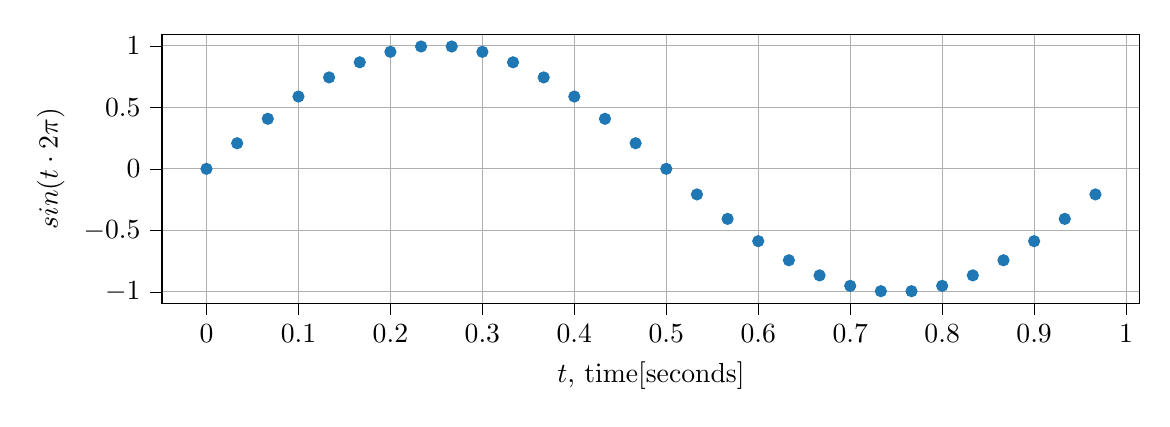
\begin{tikzpicture}

\definecolor{color0}{rgb}{0.12156862745098,0.466666666666667,0.705882352941177}

\begin{axis}[
height=5cm,
tick align=outside,
tick pos=left,
width=14cm,
x grid style={white!69.0196078431373!black},
xlabel={\(\displaystyle t\), time[seconds]},
xmajorgrids,
xmin=-0.0483333333333333, xmax=1.015,
xtick style={color=black},
y grid style={white!69.0196078431373!black},
ylabel={\(\displaystyle sin(t \cdot 2 \pi)\)},
ymajorgrids,
ymin=-1.0939740849051, ymax=1.0939740849051,
ytick style={color=black}
]
\addplot [draw=color0, fill=color0, mark=*, only marks]
table{%
x  y
0 0
0.0333333333333333 0.207911690817759
0.0666666666666667 0.4067366430758
0.1 0.587785252292473
0.133333333333333 0.743144825477394
0.166666666666667 0.866025403784439
0.2 0.951056516295154
0.233333333333333 0.994521895368273
0.266666666666667 0.994521895368273
0.3 0.951056516295154
0.333333333333333 0.866025403784439
0.366666666666667 0.743144825477394
0.4 0.587785252292473
0.433333333333333 0.4067366430758
0.466666666666667 0.207911690817759
0.5 1.22464679914735e-16
0.533333333333333 -0.207911690817759
0.566666666666667 -0.4067366430758
0.6 -0.587785252292473
0.633333333333333 -0.743144825477394
0.666666666666667 -0.866025403784438
0.7 -0.951056516295154
0.733333333333333 -0.994521895368273
0.766666666666667 -0.994521895368273
0.8 -0.951056516295154
0.833333333333333 -0.866025403784439
0.866666666666667 -0.743144825477394
0.9 -0.587785252292473
0.933333333333333 -0.4067366430758
0.966666666666667 -0.20791169081776
};
\end{axis}

\end{tikzpicture}

	% \includegraphics[width=11cm]{sineScatter}
	\caption[Sine scatter-plot]
	{Sine wave, 1Hz, sample rate 30Hz, scatter-plot}
	\label{fig:scatter}
\end{figure}



\begin{figure}[H]
	\centering
	% This file was created with tikzplotlib v0.9.14.
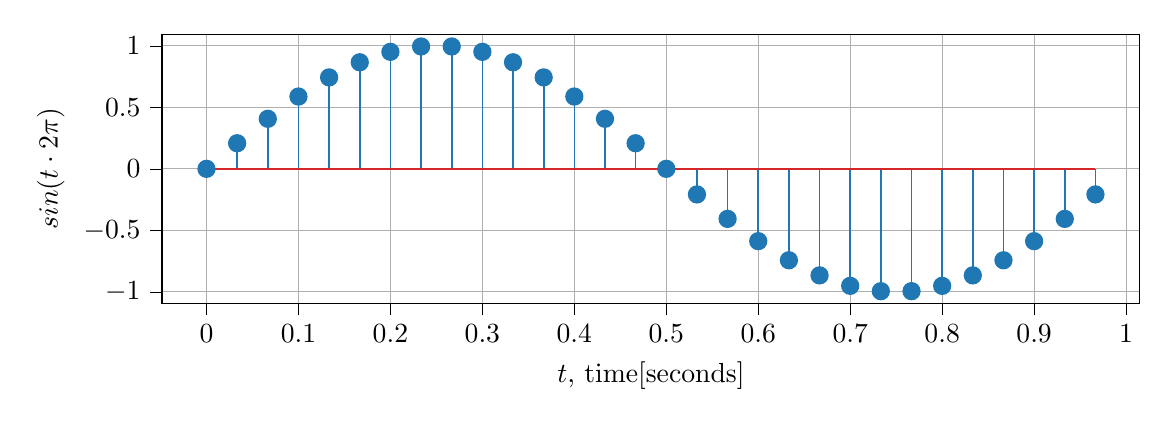
\begin{tikzpicture}

\definecolor{color0}{rgb}{0.12156862745098,0.466666666666667,0.705882352941177}
\definecolor{color1}{rgb}{0.83921568627451,0.152941176470588,0.156862745098039}

\begin{axis}[
height=5cm,
tick align=outside,
tick pos=left,
width=14cm,
x grid style={white!69.0196078431373!black},
xlabel={\(\displaystyle t\), time[seconds]},
xmajorgrids,
xmin=-0.0483333333333333, xmax=1.015,
xtick style={color=black},
y grid style={white!69.0196078431373!black},
ylabel={\(\displaystyle sin(t \cdot 2 \pi)\)},
ymajorgrids,
ymin=-1.0939740849051, ymax=1.0939740849051,
ytick style={color=black}
]
\addplot [semithick, color0]
table {%
0 0
0 0
};
\addplot [semithick, color0]
table {%
0.0333333333333333 0
0.0333333333333333 0.207911690817759
};
\addplot [semithick, color0]
table {%
0.0666666666666667 0
0.0666666666666667 0.4067366430758
};
\addplot [semithick, color0]
table {%
0.1 0
0.1 0.587785252292473
};
\addplot [semithick, color0]
table {%
0.133333333333333 0
0.133333333333333 0.743144825477394
};
\addplot [semithick, color0]
table {%
0.166666666666667 0
0.166666666666667 0.866025403784439
};
\addplot [semithick, color0]
table {%
0.2 0
0.2 0.951056516295154
};
\addplot [semithick, color0]
table {%
0.233333333333333 0
0.233333333333333 0.994521895368273
};
\addplot [semithick, color0]
table {%
0.266666666666667 0
0.266666666666667 0.994521895368273
};
\addplot [semithick, color0]
table {%
0.3 0
0.3 0.951056516295154
};
\addplot [semithick, color0]
table {%
0.333333333333333 0
0.333333333333333 0.866025403784439
};
\addplot [semithick, color0]
table {%
0.366666666666667 0
0.366666666666667 0.743144825477394
};
\addplot [semithick, color0]
table {%
0.4 0
0.4 0.587785252292473
};
\addplot [semithick, color0]
table {%
0.433333333333333 0
0.433333333333333 0.4067366430758
};
\addplot [semithick, color0]
table {%
0.466666666666667 0
0.466666666666667 0.207911690817759
};
\addplot [semithick, color0]
table {%
0.5 0
0.5 1.22464679914735e-16
};
\addplot [semithick, color0]
table {%
0.533333333333333 0
0.533333333333333 -0.207911690817759
};
\addplot [semithick, color0]
table {%
0.566666666666667 0
0.566666666666667 -0.4067366430758
};
\addplot [semithick, color0]
table {%
0.6 0
0.6 -0.587785252292473
};
\addplot [semithick, color0]
table {%
0.633333333333333 0
0.633333333333333 -0.743144825477394
};
\addplot [semithick, color0]
table {%
0.666666666666667 0
0.666666666666667 -0.866025403784438
};
\addplot [semithick, color0]
table {%
0.7 0
0.7 -0.951056516295154
};
\addplot [semithick, color0]
table {%
0.733333333333333 0
0.733333333333333 -0.994521895368273
};
\addplot [semithick, color0]
table {%
0.766666666666667 0
0.766666666666667 -0.994521895368273
};
\addplot [semithick, color0]
table {%
0.8 0
0.8 -0.951056516295154
};
\addplot [semithick, color0]
table {%
0.833333333333333 0
0.833333333333333 -0.866025403784439
};
\addplot [semithick, color0]
table {%
0.866666666666667 0
0.866666666666667 -0.743144825477394
};
\addplot [semithick, color0]
table {%
0.9 0
0.9 -0.587785252292473
};
\addplot [semithick, color0]
table {%
0.933333333333333 0
0.933333333333333 -0.4067366430758
};
\addplot [semithick, color0]
table {%
0.966666666666667 0
0.966666666666667 -0.20791169081776
};
\addplot [semithick, color0, mark=*, mark size=3, mark options={solid}, only marks]
table {%
0 0
0.0333333333333333 0.207911690817759
0.0666666666666667 0.4067366430758
0.1 0.587785252292473
0.133333333333333 0.743144825477394
0.166666666666667 0.866025403784439
0.2 0.951056516295154
0.233333333333333 0.994521895368273
0.266666666666667 0.994521895368273
0.3 0.951056516295154
0.333333333333333 0.866025403784439
0.366666666666667 0.743144825477394
0.4 0.587785252292473
0.433333333333333 0.4067366430758
0.466666666666667 0.207911690817759
0.5 1.22464679914735e-16
0.533333333333333 -0.207911690817759
0.566666666666667 -0.4067366430758
0.6 -0.587785252292473
0.633333333333333 -0.743144825477394
0.666666666666667 -0.866025403784438
0.7 -0.951056516295154
0.733333333333333 -0.994521895368273
0.766666666666667 -0.994521895368273
0.8 -0.951056516295154
0.833333333333333 -0.866025403784439
0.866666666666667 -0.743144825477394
0.9 -0.587785252292473
0.933333333333333 -0.4067366430758
0.966666666666667 -0.20791169081776
};
\addplot [semithick, color1]
table {%
0 0
0.966666666666667 0
};
\end{axis}

\end{tikzpicture}

	% \includegraphics[width=11cm]{sineStem}
	\caption[sine stem plot]
	{Sine wave, 1Hz, sample rate 30Hz, stem-plot}
	\label{fig:stem}
\end{figure}


So why don't we always do a stem- or scatter-plot? Simply because it gets too crowded with our usual sampling rates in audio. It just works with very low sampling rates or very short signals.\\
\begin{figure}[H]
	\centering
	\includegraphics[width=11cm]{stem44100}
	\caption[sine stem plot, crowded]
	{Sine wave, 1Hz, sample rate 44100Hz, stem-plot}
	\label{fig:sine1HzStemPlot}
\end{figure}
\textbf{But we should never forget that we don't actually have the values in between the dots. Digital signals are not defined between their sampled points.}

You can look at how these signals where generated and plotted \link{https://colab.research.google.com/github/hrtlacek/dspCourse/blob/master/notebooks/00\_Introduction.ipynb}{in this Notebook}

\section{What is aliasing?}
Aliasing in audio means problems caused by signals that exceed the nyquist rate.\\
The nyquist rate,let's call it $f_n$ for now, is defined by the half of the sample rate ($f_s$). So,
\begin{equation}
	f_n=\frac{f_s}{2}
\end{equation}
A digital system can only describe signals up to its nyquist rate. If we try to make signals higher than this frequency, we will fail and encounter strange effects.\\
Visually speaking, frequencies higher than nyquist fold back. So, let's assume we have a sampling rate of 100Hz. Nyquist would be at 50Hz. If we try to synthesize a sine wave with 51Hz, what we will get is a 49Hz one. If we try to make a 52Hz one, we will get 48Hz. So you see, it simply folds back. You can find an interactive example \link{https://jackschaedler.github.io/circles-sines-signals/sampling.html}{here}.

\begin{framed}
	\textbf{Video analogies}\\
	Aliasing in graphics usually means \textit{spacial} aliasing, so aliasing in the space domain. This is what we see in figure \ref{fig:spAlias}. But there is also time domain aliasing in film. It is actually more natural to think about the sampling rate in audio as the same as the frame rate in video. For some really weird effects that arise in video due to time domain aliasing see \href{https://www.youtube.com/watch?v=LVwmtwZLG88}{airplane}\footnotemark , \href{https://www.youtube.com/watch?v=GBtHeR-hY9Y}{Water experiment}\footnotemark or \href{https://www.youtube.com/watch?v=jcOKTTnOIV8}{Guitar strings}\footnotemark .
	\begin{center}
		% \centering
		\includegraphics[width=7cm]{spacialAliasing1.png}
		\captionof{figure}{Spacial aliasing in graphics. The ``frequency'' of the intended pixels is to high for the actual pixels.}
		\label{fig:spAlias}
	\end{center}
	The particularly strange effects in the airplane example above are caused by the rolling shutter of a CMOS sensor. Since it is not sampling the incoming light uniformly (at the same time) the image is distorted.
\end{framed}
\footnotetext[2]{https://www.youtube.com/watch?v=LVwmtwZLG88}
\footnotetext[3]{https://www.youtube.com/watch?v=GBtHeR-hY9Y}
\footnotetext[4]{https://www.youtube.com/watch?v=jcOKTTnOIV8}


In figure \ref{fig:cosAlias} you can see a visualization of aliasing in the time domain.

\begin{figure}[H]
	\centering
	% This file was created with tikzplotlib v0.9.14.
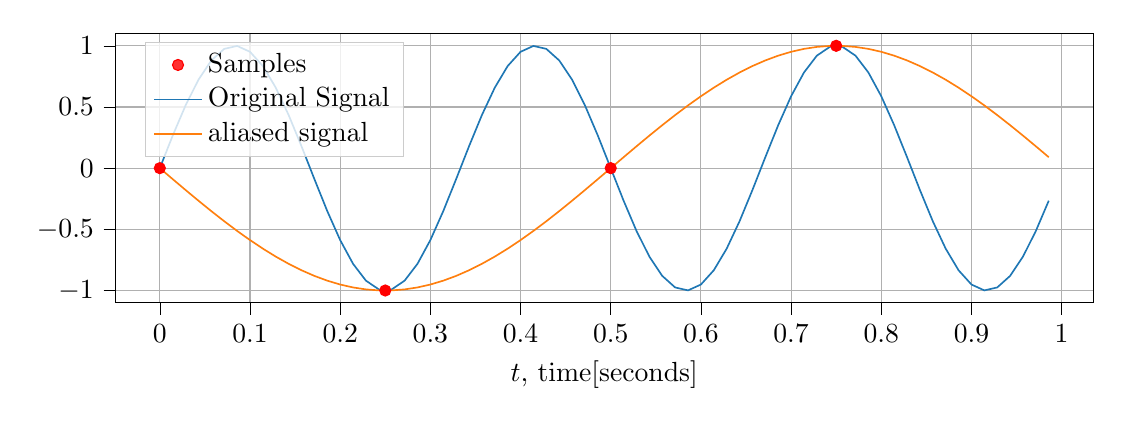
\begin{tikzpicture}

\definecolor{color0}{rgb}{0.12156862745098,0.466666666666667,0.705882352941177}
\definecolor{color1}{rgb}{1,0.498039215686275,0.0549019607843137}

\begin{axis}[
height=5cm,
legend cell align={left},
legend style={
  fill opacity=0.8,
  draw opacity=1,
  text opacity=1,
  at={(0.03,0.97)},
  anchor=north west,
  draw=white!80!black
},
tick align=outside,
tick pos=left,
width=14cm,
x grid style={white!69.0196078431373!black},
xlabel={\(\displaystyle t\), time[seconds]},
xmajorgrids,
xmin=-0.0492857142857143, xmax=1.035,
xtick style={color=black},
y grid style={white!69.0196078431373!black},
ymajorgrids,
ymin=-1.1, ymax=1.1,
ytick style={color=black}
]
\addplot [draw=red, fill=red, mark=*, only marks]
table{%
x  y
0 0
0.25 -1
0.5 3.67394039744206e-16
0.75 1
};
\addlegendentry{Samples}
\addplot [semithick, color0]
table {%
0 0
0.0142857142857143 0.266036845566675
0.0285714285714286 0.512899277405906
0.0428571428571429 0.722794863827392
0.0571428571428571 0.880595531856738
0.0714285714285714 0.974927912181824
0.0857142857142857 0.998993066541315
0.1 0.951056516295154
0.114285714285714 0.834573253721303
0.128571428571429 0.657938725939713
0.142857142857143 0.433883739117558
0.157142857142857 0.178556894798637
0.171428571428571 -0.0896393089034334
0.185714285714286 -0.351374824081343
0.2 -0.587785252292473
0.214285714285714 -0.78183148246803
0.228571428571429 -0.919527772551451
0.242857142857143 -0.990949761767935
0.257142857142857 -0.990949761767935
0.271428571428571 -0.919527772551451
0.285714285714286 -0.78183148246803
0.3 -0.587785252292473
0.314285714285714 -0.351374824081343
0.328571428571429 -0.0896393089034337
0.342857142857143 0.178556894798636
0.357142857142857 0.433883739117558
0.371428571428571 0.657938725939712
0.385714285714286 0.834573253721303
0.4 0.951056516295154
0.414285714285714 0.998993066541315
0.428571428571429 0.974927912181824
0.442857142857143 0.880595531856738
0.457142857142857 0.722794863827392
0.471428571428571 0.512899277405906
0.485714285714286 0.266036845566675
0.5 3.67394039744206e-16
0.514285714285714 -0.266036845566673
0.528571428571429 -0.512899277405906
0.542857142857143 -0.72279486382739
0.557142857142857 -0.880595531856738
0.571428571428571 -0.974927912181824
0.585714285714286 -0.998993066541315
0.6 -0.951056516295154
0.614285714285714 -0.834573253721302
0.628571428571429 -0.657938725939713
0.642857142857143 -0.433883739117559
0.657142857142857 -0.178556894798637
0.671428571428571 0.089639308903433
0.685714285714286 0.351374824081342
0.7 0.587785252292473
0.714285714285714 0.781831482468029
0.728571428571429 0.91952777255145
0.742857142857143 0.990949761767935
0.757142857142857 0.990949761767935
0.771428571428571 0.919527772551451
0.785714285714286 0.78183148246803
0.8 0.587785252292474
0.814285714285714 0.351374824081343
0.828571428571429 0.0896393089034341
0.842857142857143 -0.178556894798636
0.857142857142857 -0.433883739117558
0.871428571428571 -0.657938725939712
0.885714285714286 -0.834573253721302
0.9 -0.951056516295153
0.914285714285714 -0.998993066541315
0.928571428571429 -0.974927912181824
0.942857142857143 -0.880595531856738
0.957142857142857 -0.722794863827392
0.971428571428571 -0.512899277405907
0.985714285714286 -0.266036845566676
};
\addlegendentry{Original Signal}
\addplot [semithick, color1]
table {%
0 -0
0.0142857142857143 -0.0896393089034335
0.0285714285714286 -0.178556894798637
0.0428571428571429 -0.266036845566675
0.0571428571428571 -0.351374824081343
0.0714285714285714 -0.433883739117558
0.0857142857142857 -0.512899277405906
0.1 -0.587785252292473
0.114285714285714 -0.657938725939713
0.128571428571429 -0.722794863827391
0.142857142857143 -0.78183148246803
0.157142857142857 -0.834573253721303
0.171428571428571 -0.880595531856738
0.185714285714286 -0.919527772551451
0.2 -0.951056516295154
0.214285714285714 -0.974927912181824
0.228571428571429 -0.990949761767935
0.242857142857143 -0.998993066541315
0.257142857142857 -0.998993066541315
0.271428571428571 -0.990949761767935
0.285714285714286 -0.974927912181824
0.3 -0.951056516295154
0.314285714285714 -0.919527772551451
0.328571428571429 -0.880595531856738
0.342857142857143 -0.834573253721303
0.357142857142857 -0.78183148246803
0.371428571428571 -0.722794863827392
0.385714285714286 -0.657938725939713
0.4 -0.587785252292473
0.414285714285714 -0.512899277405906
0.428571428571429 -0.433883739117558
0.442857142857143 -0.351374824081343
0.457142857142857 -0.266036845566675
0.471428571428571 -0.178556894798637
0.485714285714286 -0.0896393089034336
0.5 -1.22464679914735e-16
0.514285714285714 0.0896393089034329
0.528571428571429 0.178556894798637
0.542857142857143 0.266036845566675
0.557142857142857 0.351374824081343
0.571428571428571 0.433883739117558
0.585714285714286 0.512899277405906
0.6 0.587785252292473
0.614285714285714 0.657938725939713
0.628571428571429 0.722794863827391
0.642857142857143 0.78183148246803
0.657142857142857 0.834573253721303
0.671428571428571 0.880595531856738
0.685714285714286 0.919527772551451
0.7 0.951056516295154
0.714285714285714 0.974927912181824
0.728571428571429 0.990949761767935
0.742857142857143 0.998993066541315
0.757142857142857 0.998993066541315
0.771428571428571 0.990949761767935
0.785714285714286 0.974927912181824
0.8 0.951056516295154
0.814285714285714 0.919527772551451
0.828571428571429 0.880595531856738
0.842857142857143 0.834573253721303
0.857142857142857 0.78183148246803
0.871428571428571 0.722794863827392
0.885714285714286 0.657938725939713
0.9 0.587785252292473
0.914285714285714 0.512899277405906
0.928571428571429 0.433883739117558
0.942857142857143 0.351374824081343
0.957142857142857 0.266036845566675
0.971428571428571 0.178556894798637
0.985714285714286 0.0896393089034337
};
\addlegendentry{aliased signal}
\end{axis}

\end{tikzpicture}

	% \includegraphics[width=\textwidth]{aliasingSine}
	\caption[Aliasing]
	{Aliasing visualized in the time domain. A sampling rate of 4 Hz is used. Therefore frequencies will fold above 2 Hz, which is the nyquist frequency. The input cosine has a frequency of 3 Hz, labeled ``Orginal Signal''. What we would get is the sampled points. If these are digital-to-analog converted, we would get what is labeled ``Aliased signal '' in this plot, so a 1 Hz cosine.}
	\label{fig:cosAlias}
\end{figure}



\begin{figure}[H]
	\begin{center}
		% This file was created with tikzplotlib v0.9.14.
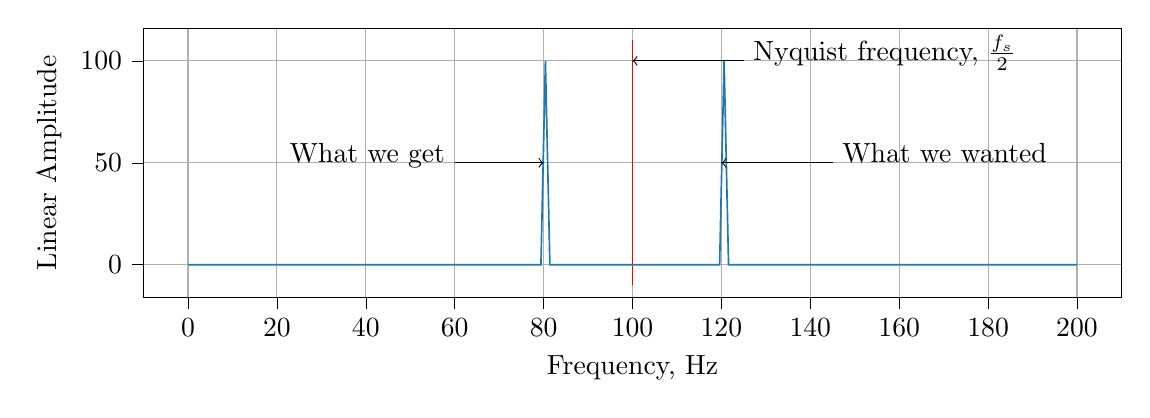
\begin{tikzpicture}

\definecolor{color0}{rgb}{0.12156862745098,0.466666666666667,0.705882352941177}

\begin{axis}[
height=5cm,
legend cell align={left},
legend style={fill opacity=0.8, draw opacity=1, text opacity=1, draw=white!80!black},
tick align=outside,
tick pos=left,
width=14cm,
x grid style={white!69.0196078431373!black},
xlabel={Frequency, Hz},
xmajorgrids,
xmin=-10, xmax=210,
xtick style={color=black},
y grid style={white!69.0196078431373!black},
ylabel={Linear Amplitude},
ymajorgrids,
ymin=-16, ymax=116,
ytick style={color=black}
]
\path [draw=red, semithick]
(axis cs:100,-10)
--(axis cs:100,110);

\addplot [semithick, color0, forget plot]
table {%
0 1.04176496399295e-13
1.00502512562814 1.22852692498498e-13
2.01005025125628 1.64146113790742e-13
3.01507537688442 5.12722440985122e-14
4.02010050251256 1.89635572984625e-13
5.0251256281407 2.09003026072463e-13
6.03015075376884 7.50942547365276e-14
7.03517587939698 3.60288211265824e-13
8.04020100502512 6.61576132530574e-13
9.04522613065327 2.76564554409926e-13
10.0502512562814 1.92358202497402e-13
11.0552763819095 1.01010880236548e-13
12.0603015075377 2.25544214791892e-13
13.0653266331658 1.8719940220499e-13
14.070351758794 1.79054616115051e-13
15.0753768844221 2.85569771117385e-13
16.0804020100502 1.52967228803167e-13
17.0854271356784 1.33152618648232e-13
18.0904522613065 3.25055345582669e-13
19.0954773869347 9.37494207957993e-14
20.1005025125628 7.44324688445693e-14
21.105527638191 1.12008567414346e-13
22.1105527638191 2.01650241098569e-13
23.1155778894472 3.85764507844166e-14
24.1206030150754 1.22134841046306e-13
25.1256281407035 1.77716093122275e-13
26.1306532663317 6.42610827635418e-14
27.1356783919598 1.09930233519008e-13
28.1407035175879 1.00447238321584e-13
29.1457286432161 2.63147928108448e-13
30.1507537688442 2.28054527984479e-14
31.1557788944724 6.16431857761929e-13
32.1608040201005 1.00717425050374e-12
33.1658291457286 6.1437309913277e-13
34.1708542713568 2.15132907111041e-13
35.1758793969849 1.13474426241041e-13
36.1809045226131 1.37983102177136e-13
37.1859296482412 9.96220009144911e-14
38.1909547738693 1.4885545103043e-13
39.1959798994975 5.57427005466418e-14
40.2010050251256 1.96442650341593e-13
41.2060301507538 7.58989451556911e-14
42.2110552763819 1.12263009547582e-13
43.21608040201 1.02050855855012e-13
44.2211055276382 4.47725140338821e-13
45.2261306532663 1.94400582025006e-13
46.2311557788945 2.21580056477014e-13
47.2361809045226 1.06863139747685e-13
48.2412060301507 2.26265351437867e-13
49.2462311557789 2.48590493456595e-13
50.251256281407 1.75879195070945e-13
51.2562814070352 1.86379320904195e-13
52.2613065326633 1.26339595925153e-13
53.2663316582914 3.61765550615109e-13
54.2713567839196 1.26104522344852e-13
55.2763819095477 6.32223321930097e-13
56.2814070351759 2.80114763394157e-13
57.286432160804 3.74598856610979e-13
58.2914572864322 1.83294213991289e-13
59.2964824120603 3.16493249884931e-13
60.3015075376884 1.32348658780032e-13
61.3065326633166 2.93542065695892e-13
62.3115577889447 3.94552579858922e-13
63.3165829145729 5.72370092402213e-13
64.321608040201 3.21950119807266e-13
65.3266331658291 5.95757284561417e-13
66.3316582914573 9.07334943155623e-14
67.3366834170854 4.52510054150999e-13
68.3417085427136 1.98436432015242e-13
69.3467336683417 3.94453972800867e-13
70.3517587939699 2.44419234067847e-13
71.356783919598 2.52377912116451e-13
72.3618090452261 4.94239698060309e-13
73.3668341708543 1.04185395358712e-13
74.3718592964824 3.17340701978095e-13
75.3768844221105 2.86332531789509e-13
76.3819095477387 1.49001844677157e-13
77.3869346733668 1.36394683724063e-13
78.391959798995 3.39880727020675e-14
79.3969849246231 5.07478435387728e-13
80.4020100502512 100
81.4070351758794 4.87193769432429e-13
82.4120603015075 2.61411391347904e-13
83.4170854271357 7.76276232514779e-14
84.4221105527638 3.80535453173215e-13
85.4271356783919 4.62076194956417e-14
86.4321608040201 3.00411173126564e-13
87.4371859296482 3.83741230136667e-13
88.4422110552764 1.00186303096534e-12
89.4472361809045 4.8640340558884e-13
90.4522613065326 3.29485093688873e-13
91.4572864321608 5.57159265566705e-13
92.4623115577889 2.34713721542699e-13
93.4673366834171 9.82265840119626e-14
94.4723618090452 6.23132215485983e-14
95.4773869346734 5.60460276382572e-13
96.4824120603015 5.59103393893974e-13
97.4874371859296 5.26433104938941e-13
98.4924623115578 3.65152025209291e-13
99.4974874371859 3.57935787429034e-13
100.502512562814 1.43399997116854e-13
101.507537688442 3.57935787429034e-13
102.51256281407 3.65152025209291e-13
103.517587939698 5.26433104938941e-13
104.522613065327 5.59103393893974e-13
105.527638190955 5.60460276382572e-13
106.532663316583 6.23132215485983e-14
107.537688442211 9.82265840119626e-14
108.542713567839 2.34713721542699e-13
109.547738693467 5.57159265566705e-13
110.552763819095 3.29485093688873e-13
111.557788944724 4.8640340558884e-13
112.562814070352 1.00186303096534e-12
113.56783919598 3.83741230136667e-13
114.572864321608 3.00411173126564e-13
115.577889447236 4.62076194956416e-14
116.582914572864 3.80535453173215e-13
117.587939698492 7.7627623251478e-14
118.592964824121 2.61411391347904e-13
119.597989949749 4.87193769432429e-13
120.603015075377 100
121.608040201005 5.07478435387728e-13
122.613065326633 3.39880727020675e-14
123.618090452261 1.36394683724063e-13
124.623115577889 1.49001844677157e-13
125.628140703518 2.86332531789509e-13
126.633165829146 3.17340701978095e-13
127.638190954774 1.04185395358712e-13
128.643216080402 4.94239698060309e-13
129.64824120603 2.52377912116451e-13
130.653266331658 2.44419234067847e-13
131.658291457286 3.94453972800867e-13
132.663316582915 1.98436432015242e-13
133.668341708543 4.52510054150999e-13
134.673366834171 9.07334943155623e-14
135.678391959799 5.95757284561417e-13
136.683417085427 3.21950119807266e-13
137.688442211055 5.72370092402213e-13
138.693467336683 3.94552579858922e-13
139.698492462312 2.93542065695892e-13
140.70351758794 1.32348658780032e-13
141.708542713568 3.16493249884931e-13
142.713567839196 1.83294213991289e-13
143.718592964824 3.74598856610979e-13
144.723618090452 2.80114763394157e-13
145.72864321608 6.32223321930097e-13
146.733668341709 1.26104522344852e-13
147.738693467337 3.61765550615109e-13
148.743718592965 1.26339595925153e-13
149.748743718593 1.86379320904195e-13
150.753768844221 1.75879195070945e-13
151.758793969849 2.48590493456595e-13
152.763819095477 2.26265351437866e-13
153.768844221106 1.06863139747685e-13
154.773869346734 2.21580056477014e-13
155.778894472362 1.94400582025006e-13
156.78391959799 4.47725140338821e-13
157.788944723618 1.02050855855012e-13
158.793969849246 1.12263009547582e-13
159.798994974874 7.5898945155691e-14
160.804020100502 1.96442650341593e-13
161.809045226131 5.57427005466417e-14
162.814070351759 1.4885545103043e-13
163.819095477387 9.96220009144911e-14
164.824120603015 1.37983102177136e-13
165.829145728643 1.13474426241041e-13
166.834170854271 2.15132907111041e-13
167.839195979899 6.14373099132769e-13
168.844221105528 1.00717425050374e-12
169.849246231156 6.16431857761929e-13
170.854271356784 2.28054527984479e-14
171.859296482412 2.63147928108448e-13
172.86432160804 1.00447238321584e-13
173.869346733668 1.09930233519008e-13
174.874371859296 6.42610827635418e-14
175.879396984925 1.77716093122275e-13
176.884422110553 1.22134841046306e-13
177.889447236181 3.85764507844166e-14
178.894472361809 2.01650241098569e-13
179.899497487437 1.12008567414346e-13
180.904522613065 7.44324688445693e-14
181.909547738693 9.37494207957992e-14
182.914572864322 3.25055345582669e-13
183.91959798995 1.33152618648232e-13
184.924623115578 1.52967228803167e-13
185.929648241206 2.85569771117385e-13
186.934673366834 1.79054616115051e-13
187.939698492462 1.8719940220499e-13
188.94472361809 2.25544214791892e-13
189.949748743719 1.01010880236548e-13
190.954773869347 1.92358202497402e-13
191.959798994975 2.76564554409926e-13
192.964824120603 6.61576132530574e-13
193.969849246231 3.60288211265824e-13
194.974874371859 7.50942547365277e-14
195.979899497487 2.09003026072463e-13
196.984924623116 1.89635572984625e-13
197.989949748744 5.12722440985122e-14
198.994974874372 1.64146113790741e-13
200 1.22852692498498e-13
};
\draw[->,draw=black] (axis cs:125,100) -- (axis cs:100,100);
\draw (axis cs:125,100) node[
  scale=1,
  anchor=base west,
  text=black,
  rotate=0.0
]{Nyquist frequency, $\frac{f_s}{2}$};
\draw[->,draw=black] (axis cs:145,50) -- (axis cs:120,50);
\draw (axis cs:145,50) node[
  scale=1,
  anchor=base west,
  text=black,
  rotate=0.0
]{What we wanted};
\draw[->,draw=black] (axis cs:60,50) -- (axis cs:80,50);
\draw (axis cs:60,50) node[
  scale=1,
  anchor=base east,
  text=black,
  rotate=0.0
]{What we get};
\end{axis}

\end{tikzpicture}

		% \includegraphics[width = \textwidth]{aliasingFreqDomain.png}
		\caption[Aliasing in the Frequency Domain]
		{Here we can see the phenomenon of aliasing in the frequency domain. We try to synthesize a sine wave at 120Hz. At a sampling rate of 200 Hz, this is not possible, nyquist is at 100 Hz. What we actually get is a sine wave at about 80Hz. In this plot, the nyquist frequency is marked with the red line. Please note that the distance between the red line to both peaks is identical. This is why the phenomenon is also called \textit{fold-back}.}
		\label{fig:aliasingFreqDomain}
	\end{center}
\end{figure}


But how is the aliased frequency calculated? To get a correct result also if you go 2 or more times past the Nyquist frequency, and still be correct in phase, please look at \link{https://colab.research.google.com/drive/10NRGmmLRGxy\_3j7ecGKcME0gkQKmCDOW}{this Notebook}. For the case where we go only once over the Nyquist Frequency we can just calculate:

\begin{equation}
	f_a = f_s-f_o
\end{equation}
Where $f_a$ is the Frequency we will hear, $f_o$ is the intended frequency and $f_s$ is the sampling rate. 
\bgInfo{
For cases where we pass Nyquist multiple times things start to get a bit complicated. In case we went over Nyquist odd times we can use the following Equation making use of the modulo. That is this equation os valid between $f_n$ and $f_s=2f_n$, between $3f_n$ and $4f_n$ and so on:


\begin{equation}
	f_a = (fs-f_o) mod  \frac{f_s}{2}
\end{equation}

otherwise we have to use the following Equation:
\begin{equation}
	f_a = f_o mod  \frac{f_s}{2}
\end{equation}

}

\section{Scaling and Mapping Signals}
It is an important skill to be able to scale signals from one range to another. We need it a lot and we will be able to think about signals more easily if we mastered this task. It's actually quite simple, we just have to imagine the signals visually.\\
So what exactly do we have to do here? We are confronted with the following problem: Given some signal, say, a sine wave with its maximum at the value 1 and its minimum at the value -1. How to bring it to a different range, say, 0-10?\\
It helps me a lot to solve this problem in two parts: first get the input in the range 0-1, then from there go to the desired range. What can we do to the signal? Let's take a sine wave like the one in Figure ~\ref{fig:aSine}. Well we can add and subtract to move the wave vertically, so let's add 1 to move it up, have a look at Figure~\ref{fig:aShiftedSine}.

\begin{figure}[H]
	\centering
	\includegraphics[width=11cm]{stdSine.png}
	\caption[a sine wave]
	{a sine wave}
	\label{fig:aSine}
\end{figure}

\begin{figure}[H]
	\centering
	\includegraphics[width=11cm]{sinePlusOne.png}
	\caption[a sine wave]
	{the same sine wave, 1 added to a each sample, therefore shifted upwards.}
	\label{fig:aShiftedSine}
\end{figure}

So we can move signals around by adding constant values. We can scale them by multiplication. So if we take our sine that now ranges from 0 to 2 and multiply it by 0.5, we get whats in figure \ref{fig:sine01}.

\begin{figure}[H]
 	\centering
 	\includegraphics[width=11cm]{sine01.png}
 	\caption[sine 0 to 1]
 	{Sine with a range of 0-1. Obtained by taking a sine wave, adding 1 and dividing by two afterwards.}
 	\label{fig:sine01}
 \end{figure}

\hspace{1cm}

Using what we got now in figure \ref{fig:sine01}, we can just multiply by 10, easy! Beware that there are always multiple solutions to this kind of a problem. Try to find another one for the problem above!

\begin{question}
Let's take a sine wave that has it's minimum at 2 and it's maximum at 5. What do we have to do to get it into a -1 to 1 range?
\end{question}
\begin{Answer}
We could subtract 3.5 to center the wave around zero first. Afterwards we take care of the amplitude by multiplying by $\frac{2}{3}$ (since the initial wave has a peak-to-peak amplitude of three and we want a peak-to-peak amplitude of 2)
\end{Answer}



\section{What's DC-Offset?}

What we did above by adding a constant value to a signal can be called adding DC-offset (``Gleichspannungsversatz''), DC-Bias or a DC component. These are different words for the same thing.\\
DC-offset can also be encountered in signals we recorded (caused by old or broken equipment mainly). But we have seen that we can also generate DC-offset.\\
To state it again clearly:
\begin{framed}
DC-Offset is a constant value over time, or a constant offset from the zero value in Y. So for example in figure \ref{fig:sine01} we see a DC-offset of 0.5 since subtracting this value would center the wave around 0.
\end{framed}
If we try to think how this kind of signal looks in the frequency domain we find that it is energy at 0Hz. In figure \ref{fig:dcViz} you can see a couple of cosine waves plotted. This should hep imagine that a constant signal, a signal that does not move a all, can be described by a cosine with 0 Hz and a certain amplitude.

\begin{figure}[h!]
	\centering
	\includegraphics[width=11cm]{dcOffsetViz}
	\caption[Cosines to DC]
	{Cosines with different very low frequencies approaching 0Hz, so DC offset.}
	\label{fig:dcViz}
\end{figure}

Let's quickly state this differently, so we can appreciate the surprising connections between DC-offset and an impulse. A DC-offset signal is a signal consisting of constant values, so for example $\{...,1,1,1,1,1,1,...\}$. Its spectrum is a single peak at 0Hz, so the spectrum's values look like $\{..., 0,0,0,1,0,0,0,...\}$\footnote{Why is the $1$, so the 0 Hz component not at the beginning of the list? Or is it not 0 Hz? The 1 is supposed to be at 0Hz, and it is centered in this list because doing an FFT actually always gets us a two-sided spectrum. You can ignore this fact until the FFT chapter, and pretend that the list starts with 1 (which wouldn't be wrong also). }


\begin{figure}[H]
	\begin{center}
		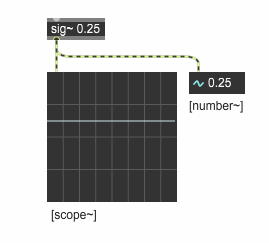
\includegraphics{dcPd.png}
		\caption[Dc-offset in Max]
		{One of the ways to generate a DC signal in Max.}
		\label{fig:dcOffsetPD}
	\end{center}
\end{figure}




% \comm{explanations and visualizations missing}

\section{What's an Impulse?}

Impulses are very useful signals. We can produce an impulse using the \pd{click\textasciitilde} object.

\begin{figure}[H]
	\begin{center}
		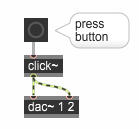
\includegraphics{dirac.png}
		\caption[The click object]
		{The \pd{click\textasciitilde} object produces an impulse if we send it a \texttt{bang}.}
		\label{fig:impulseInPd}
	\end{center}
\end{figure}
\bgInfo{
Different people will define what's an impulse in different ways:
\begin{itemize}
	\item A sound engineer might tell you, that clapping your hands or shooting with a gun creates an impulse
	\item a mathematician will maybe give you the definition of the \textit{dirac delta function}. A dirac function is a continuous function having infinite height and being infinitely short. Its integral (area under the curve) is 1.
	\item Somebody working with discrete (so digital) signals will give you rather the definition of the Kronecker delta function\footnote{It's very common and kind of wrong to call digital impulses "dirac functions" or "dirac impulses". Sometimes people like to use "big" words. So instead of saying "impulse", they say "dirac delta function". Dirac delta functions have importance in mathematics and analysis. But since they have infinite value and are infinitely short they can't exist in reality. They are a theoretical idea. Therefore, more often than not, the term is used a bit incorrectly in an audio context.}:
	\begin{equation}
		\delta(i) = \begin{cases}
0, & \mbox{if } i \ne 0  \\
1, & \mbox{if } i=0 \end{cases}
	\end{equation}
\end{itemize}


}

For us, strictly speaking, an impulse will be a signal that contains only zeros, but one sample with the value one (so we will mean the Kronecker delta function if we say 'impulse'). We can see such an impulse in figure \ref{fig:unitImpulse}. On the x-axis, we have the time in samples\footnote{Don't be irritated by the fact that the sample numbers on the x-axis are ranging from $-5$ to $5$. You can just as well imagine them going from 0 to 10 or 1 to 11. It doesn't really matter. However, this way of displaying an impulse is very common since if the impulse is filtered, it's symmetry is an important factor.}.


\begin{figure}[H]
	\begin{center}
		\includegraphics[width = \textwidth]{unitImpulse.png}
		\caption{unit impulse function}
		\label{fig:unitImpulse}
	\end{center}
\end{figure}

So in the time domain, an impulse's samples have the values $\{...,0,0,0,1,0,0,0,...\}$. If we look at it's spectrum, we will find that it contains all frequencies, there is just a flat line in the spectrum (you can see an impulse's spectrum in figure \ref{fig:impToDc} also.). The spectrum has a \textit{constant value}, something like $\{..,1,1,1,1,1,1,...\}$. Do these two lists look familiar? Right, it is exactly the opposite of the DC-offset signal.



\section{How to describe audio mathematically}

If we want to talk about signals, or if we want to analyze them, it is often useful to look at the problem mathematically. First, let's introduce some conventions. They might look unfamiliar or complicated. But in fact it is not very complicated and knowing these conventions makes it easy to communicate (e.g. reading scientific papers about our topics or explaining something to another person).

\subsection{signals}

Usually we describe a \textit{digital} signal by a name, say $x$, (but you can call it however you want). If we want to talk about the individual samples, or values of the (mono) signal, we can use a subscript or parenthesis. So if the fifth sample of $x$ is 1, we could write:

\begin{equation}
	x_5=1
\end{equation}
or
\begin{equation}
	x(5)=1
\end{equation}
Oftentimes we like to talk about a signal more generally and we use $n$ as a place holder for this index, so we might write $x_n$, meaning the nth sample of $x$.

\subsubsection{sine waves}
We use sine waves a lot. The syntax can get a bit overwhelming at first, so let's quickly explain what's going on in a standard sine wave oscillator.
\begin{equation}
	x(t) = A \cdot sin(2\pi f t + \phi)
\end{equation}
Where $f$ is the frequency in Hertz and $t$ is the time in seconds. $\phi$ Is a (possibly constant) phase offset and $A$ can be used to scale the whole thing. Since cosine and sine have their peaks at -1 and 1, $A$ will be the amplitude. If $A$ is set to 0.5, the resulting signal will have it's peaks at -0.5 and 0.5. \\
The upper equation is rather complete. Most of the time, we will just ignor the phase and the amplitude and just write:
\begin{equation}
	x(t) = sin(2\pi f t )
\end{equation}

Sometimes, we will simplify even more and just write $sin(a)$ or $sin(b)$ or similar.\\
\begin{mdframed}[backgroundcolor=black!10,rightline=false,leftline=false]
In literature, we sometimes encounter $x(t) = sin(t \cdot \omega)$. $\omega$ stands for a ``frequency''(actually for the rotational speed) in \textit{radians per second}. $2\pi$ radians per second are 1 Hz and we can therefore convert radians per second to frequency, $v$, with:
\begin{equation}
  	v = \omega / 2\pi
  \end{equation}
This notation is only covered since it is very common, but it will not be used here, since it is considered more intuitive to work with frequency in Hz.
\vspace{0.5cm}

\textbf{What is actually the significance of using either $sin$ or $cos$?}\\
In most cases for us, this does not matter at all. The difference between sine and cosine is just in phase. Since we are most of the time describing a sine (or cosine) wave oscillator as a function of time we can think of the sine as a slightly time shifted version of the cosine and vice versa. This minute difference is not audible. \\
That being said, there are certain formulas that consist of sine and cosine terms, and that only work that particular way. For example, Euler's famous formula, $e^{ix}=cos(x)+i\cdot sin(x)$. We can't interchange $sin$ and $cos$ here.


\end{mdframed}
% \comm{work in progress.}

\subsection{systems}
There are many ways to describe systems. Digital LTI systems (Linear, time invariant Systems) can be described using
\begin{itemize}
	\item difference equations
	\item Block diagrams
	\item Transfer Functions
	\item and other things.
\end{itemize}

For us, the most important ways to describe a system are block diagrams and difference equations.

\subsection{systems}

There are multiple ways in which we can describe linear time invariant (LTI) systems. We will talk more about this in chapter \ref{chap:filters}. Here, we will just look at how \textit{difference equations} work. These are one possibility to describe a digital LTI system. They are the discrete equivalent of difference equations. It's really not that complicated:
\begin{equation}
	y(n) = x(n)
\end{equation}
Would be an equation that describes a system that does nothing. it takes the input sample, $x(n)$ does nothing and defines the output sample $y(n)$ with it.
Another really simple system would multiply its input by two:
\begin{equation}
	y(n) = x(n)\cdot 2
\end{equation}
It's getting interesting if we start playing with the index:
\begin{equation}
	y(n) = x(n-1)
\end{equation}
Is a delay by one sample.
\begin{equation}
	y(n) = x(n)+x(n-1)
\end{equation}
Takes it's input sample and the previous input sample, adds them together and spits it out. Can you imagine what this does? We'll get to it in chapter \ref{chap:filters}...

This is just a preview, but it really gets interesting if we start working with feedback:
\begin{equation}
 	y(n) = x(n)+y(n-1)
 \end{equation}


\section{Message Domain/Signal Domain}
This is not Max/MSP specific although it might sound like it.
In Max/MSP we can have audio signals. Audio signals are processed in buffers. They are just numbers, but these numbers are calculated at a rate of 44100 Hz \textit{all the time} if we choose to have our sample rate at 44100 Hz.\\
Messages on the other hand are not calculated that often and not all the time. Messages are processed \textit{on demand}. They are event based. This means that, for example, if we hit a note on our midi keyboard or enter a number in a \pd{Numberbox} this \textit{event} will pass through its following objects \textit{once}. Have a look at figure ~\ref{fig:mesSig} or at the patcher. Also note that Max helps us in understanding if we deal with message or signal domain:

\begin{itemize}
	\item Max is indicating the signal domain with colored thicker patch cords
	% \item signal domain cables offer 
	\item objects that deal with the signal domain have a tilde (\textasciitilde ) at the end of their name.
\end{itemize}
 % by indicating the signal domain with thicker patch cords and black inlets/outlets on the objects (look closely).

\begin{figure}[h!]
	\centering
	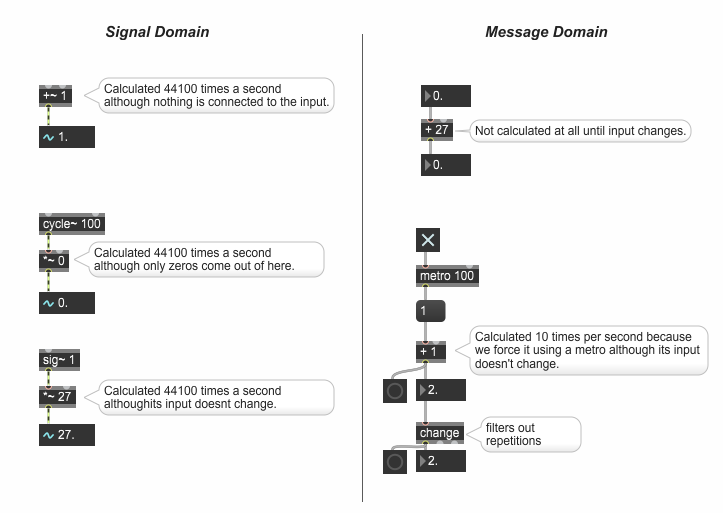
\includegraphics[width=\textwidth]{messageDomainSignalDomain}
	\caption[message domain vs. signal domain]
	{The patcher \href{./patchers/00\_introduction/00\_messageDomainSignalDomain.maxpat}{\texttt{00\_messageDomainSignalDomain.maxpat}} should demonstrate the differences between message domain and signal domain in Max/MSP.}
	\label{fig:mesSig}
\end{figure}

\paragraph{How is this not specific to Max/MSP?} The key points here are not specific to this programming language. If we, for example adjust the volume of a track in pro tools or ableton live or similar, then the information of our fader movement will also be in some kind of message domain.\\
One key aspect here is: some kind of conversion between the two is necessary if we want to switch between them. If we want to control the volume of an audio signal from the message domain we have a problem: we will get noisy output since the message domain is not running at sample rate. Look at a naive attempt to controlling the amplitude of a sine wave:

\begin{figure}[H]
	\centering
	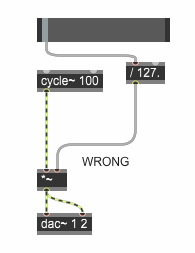
\includegraphics{ampWrong}
	\caption[patcher \texttt{00\_ampWrong.maxpat}]
	{The patcher \href{./patchers/00\_introduction/00\_ampWrong.maxpat}{\texttt{00\_ampWrong.maxpat}}}
	\label{fig:ampWrongRight}
\end{figure}


And let's look at what kind of waveform it will produce:

\begin{figure}[H]
	\centering
	\includegraphics[width=\textwidth]{ampWrongViz}
	\caption[Amplitude control, message domain ]
	{This is a cosine wave at 20 Hz and the message domain running at 100 millisecond interval to make the effect more extreme and visible}
	\label{fig:msgDomainAmpControl}
\end{figure}


This is a problem, since the sudden jumps produce clicks, crackling or zipper noise (reproduce or open the patcher and hear it for yourself!). These clicks are caused by the fact that the message domain just doesn't produce
the numbers at the rate of the sampling rate. It's too slow, so to speak.\\
In Max/MSP (but also in general) this problem can be solved by interpolation. Max/MSP offers the \pd{line\textasciitilde} object for this situation. It can be used to create signals at sampling rate and we can tell it to ramp to a specified value in a given amount of time. In figure \ref{fig:ampRight} we see it ramping to any value that comes from the \pd{/ 127.} object within 20 milliseconds\footnote{20ms is just an example. It is a reasonable time for this kind of interpolation but really, it is just an example. It could just as well be 50 ms.}. This interpolation reduces the clicks and noise dramatically. Note that the output of \pd{line\textasciitilde} is in the signal domain (thick cable).

\begin{figure}[H]
	\centering
	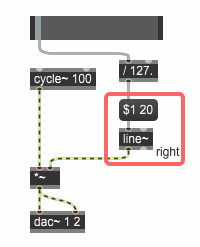
\includegraphics{ampRight}
	\caption[Amplitude control, signal domain]
	{Controlling the amplitude of an oscillator. The interpolation done with \pd{line\textasciitilde} suppresses clicks. }
	\label{fig:ampRight}
\end{figure}


\section{Key Points}
\begin{itemize}
	\item Make sure you understand and know the mathematical notation. It will be how we talk in the remaining chapters.
	\item Make sure you understand what aliasing means in audio.
	\item Make sure you are comfortable with basic mathematical operations on signals, such as adding constants and multiplying with constants
	\item Make sure you understand the difference between message and signal domain and the problem with using a message domain ``signal'' controlling an audio stream.
	\item Make sure you know what the spectrum and time domain signal of an impulse and DC-Offset look like.
\end{itemize}


\newpage
% \pagestyle{fancy}
%Inhaltsverzeichnis
\tableofcontents

\newpage
%Seitennummerierung neu beginnen, Zahlen [arabic], röm.Zahlen [roman,Roman], Buchstaben [alph,Alph]
% \pagenumbering{arabic}

% pagestyle für gesamtes Dokument aktivieren
% \pagestyle{fancy}


\newpage
% ---------SEMESTER3----------
\part{Semester 3} % (fold)
\label{prt:semester3}

%!TEX root = main.tex

\chapter{Sampling, waveshaping, and non-linearity}
\label{Waveshaping}

\begin{center}
\begin{figure}[h!]
\tikzset{concept/.append style={fill={none}}}
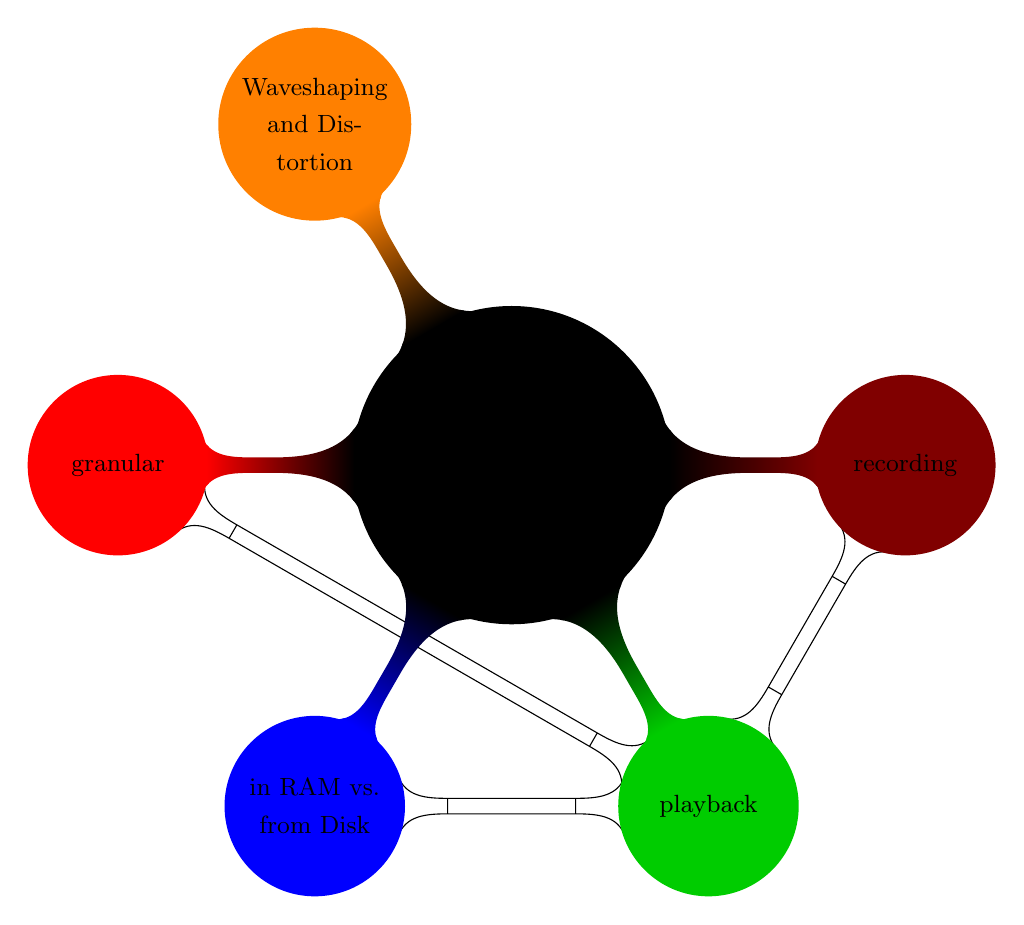
\begin{tikzpicture}
  \path[mindmap,concept color=black,text=black]
    node[concept] {Sampling}
    [clockwise from=0]
    child[concept color=red!50!black] {node[concept] (rec) {recording} }
    child[concept color=green!80!black] {node[concept] (pla) {playback} }
    %   [clockwise from=90]
    %   child { node[concept] {algorithms} }
    %   child { node[concept] {data structures} }
    %   child { node[concept] {pro\-gramming languages} }
    %   child { node[concept] {software engineer\-ing} }
    % }
    child[concept color=blue] { node[concept] (ram) {in RAM vs. from Disk}[clockwise from=-30]}
    child[concept color=red] { node[concept] (gra) {granular} }
    child[concept color=orange] { node[concept] {Waveshaping and Distortion} };

\begin{pgfonlayer}{background}
	% \draw [draw=green,fill=black, decorate,decoration=circle connection bar]
    \draw [circle connection bar]
    % \path (rec) to[circle connection bar] (pla)
      (rec) edge (pla)
      (gra) edge (pla)
      (ram) edge (pla)
      ;
  \end{pgfonlayer}

\end{tikzpicture}
\caption{Lecture Contents}
\end{figure}
\end{center}

% \section{Notizen}

% Waveshaping generell.

% Evt. Subtraktiver Synth am ende.

% Zusammenhang waveshaping, distortion. lookup table, sampling, wavescanning.

% Waveshaping = modulation \cite[p.~257]{farnell_designing_2010}

% chebyshev

% \glqq{}intermod. distortion \grqq{} , vgl. miller puckette, \\
% http://msp.ucsd.edu/techniques/latest/book-html/node78.html

% middle term! ( (a+b)**2 = a**2 +2ab +b**2 )




% beispiele:
% sinus
% vllt:\\
% dyn. non-linear functions




% \section{Uebersicht}
% Zunächst: Sampling, dann lineare transfer function.

% \begin{enumerate}
% 	\item übersicht: fragen wies geht, wie ist es mit Max/MSP?
% 	\item HÜ ankündigen
% 	\item neue abstraction: z-1
% 	\item Raetsel
% 	\item Wo letztes mal stehngeblieben? Poly syth fertig?
% 	\item linearität erklären. Nun Nichtlinearität.
% 	\item wavetable/lookup wiederholung
% 	\item Lookup als waveshaping/distortion
% 	\item waveshaping durch processing vs. durch lookuptable
% 	\item durchrechnen
% 	\item chebyshev
% 	\item Sampling (Ram nicht Ram)
% 	\item send and receive von GUI f. Hausübung
% \end{enumerate}

\section{Waveshaping}
Wikipedia quote, page ``waveshaper'':\\
\glqq{}The mathematics of non-linear operations on audio signals is difficult, and not well understood.\grqq{}
Waveshaping means distortion. It adds overtones, take a look at figure ~\ref{fig:waveshapedSIne}.


\begin{figure}[h!]
	\centering
	\includegraphics[width=11cm]{waveShapedSine.png}
	\caption[Wave shaped sine oscillator]
	{A sine wave has been generated and waveshaping was applied to add overtones.}
	\label{fig:waveshapedSIne}
\end{figure}


\begin{figure}[h!]
	\centering
	\includegraphics[width=11cm]{tanhTime.png}
	\caption[Distorted sine, time domain]
	{The same as the spectrogram above, but in the time domain. We can see the input sine wave and the slightly distorted output. It may look like just the amplitude has changed, but the sine's actual \textit{shape} has changed slightly}
	\label{fig:tanhTimeDom}
\end{figure}

\subsection{The simplest case: a linear Transfer function. } % (fold)
\label{sub:linearTrans}
See \ref{fig:linfunct}. A linear transfer function is used as a lookup table for a sinosoidal input.

\begin{figure}[H]
	\begin{center}
		\includegraphics[scale = 1]{img/waveShapingVisual.png}
		\caption{Linear Transfer function}
		\label{fig:linfunct}
	\end{center}
\end{figure}
A transfer function in the sense of a waveshaper (a ``transfer function'' might also mean frequency response in other contexts) is a simple look-up function. \
Waveshaping means to use an input wave to \textit{look up} values in a table or function. A linear transfer function, let's call it $l$, can result in no change, for example, it might return $l(x)=x$. \
This means, that whatever value we pass in, we get the same value out.\
Other linear transfer functions might \textit{only} change the amplitude. For example $f(x)=x \cdot \frac{1}{2}$. That doesn't seem very interesting. But it might explain the term ``linear''. A transfer function is linear if it looks like a line if we plot it. Look at figure \ref{fig:linears}.

\begin{figure}[h!]
	\centering
	\includegraphics[width=15cm]{linearFunctions.png}
	\caption[Linear Transfer functions]
	{A couple of linear transfer functions and their corresponding effects demonstrated using a sine wave. From left to right: multiplication by 0.5, so attenuation by about 6dB, inversion, and the ``do-nothing''-function.}
	\label{fig:linears}
\end{figure}


Non-liner transfer functions behave differently. They map their input to other values, such as $f(x) = x^2$. And if we plot then, they don't look like a line.  You can also look at figure \ref{fig:farnellWaveShaping} in order to understand what's happening. We again see a linear transfer function but also a non linear one.
\begin{figure}[H]
	\centering
	\includegraphics[width=13cm]{waveshapingVizFarnell.png}
	\caption[farnell wave shaping visualization]
	{A waveshaping visualization taken from \cite{farnell_designing_2010}}
	\label{fig:farnellWaveShaping}
\end{figure}

But let's get back to our square function, since it's simpler and we will find some surprising results when analyzing it. Let's first simply plot it too.


\begin{figure}[H]
	\begin{center}
		\includegraphics[width = 14cm]{img/squareFunction.png}
		\caption{The function $f(x)=x^2$}
		\label{fig:square}
	\end{center}
\end{figure}

% subsection subsection_name (end)

\video{
What does applying a curve to every pixel of a video or image do? Is this even something people do? Of course! Think of contrast curves, below is an example from photoshop. Beware that video is working with unipolar input values and audio with bipolar inputs.
\begin{center}
  \includegraphics[width=8cm]{photoshop.png}
  \captionof{figure}{Contrast curve in photoshop}
  \label{fig:photoshop}
\end{center}
}

\subsection{Simple non-linearity: \(X ^2\)} % (fold)
\label{sub:nonLinearTrans}

So let's analyze what happens if we use this function for waveshaping. Here it is again:

\begin{equation}
f(x) = x ^ 2
\end{equation}



% \fbox{
%   \parbox{\textwidth}{
%     Ein polynom geradzahliger ordnung \(n\) als Transferfunktion produziert immer alle geradzahligen obertöne von \(n\) bis 0, exklusive der grundfrequenz (da ja auch ungerade, 1 ist eine ungerade zahl).\\
% Ein polynom ungeradzahliger ordnung \(n\) als Transferfunktion produziert immer alle ungeradzahligen obertöne von \(n\) bis 1, also der grundfrequenz.
%   }
% }
Let's simply listen to what's happening, building it in pd:

\begin{figure}[H]
	\begin{center}
		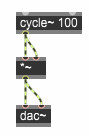
\includegraphics[width = 3cm]{img/pd_square.png}
		\caption{The square function in pure data, using a 100Hz sine as a test signal. What do you hear?}
		\label{fig:squarePd}
	\end{center}
\end{figure}



And we can simply plot what happened if we apply the function before also trying to understand analytically:


\begin{figure}[H]
	\begin{center}
		\includegraphics[width = 14cm]{img/sinSquared.png}
		\caption{Applying the square function to an input sine wave.}
		\label{fig:sinSquared}
	\end{center}
\end{figure}


Weird, the input seems to double in frequency (did you hear that?). Let's try to understand what's happening.\

So we calculate what happens if we send a cosine through this function, so let's take:

\begin{equation}
x = cos(\omega)
\end{equation}
wit arbitrary $\omega$. We can just ignore $\omega$ here for a while. Usually, there should be some indexing variable in the cosine function if we want to describe an oscillator that moves over time, but let's also skip that.\\
So applying our square function we of course get:
\begin{equation}
y = cos(\omega)^2
\end{equation}
This again results in:
\begin{equation}
y = cos(\omega) \cdot cos(\omega)
\end{equation}
So far so trivial. Note that a multiplication of two oscillators is called \textit{Amplitude Modulation} (actually, in this case we encounter ``Ring Modulation'', but let's ignore that also), and we know things about Amplitude modulation, namely:\

\fbox{
  \parbox{\textwidth}{
  When multiplying two oscillators, we get sum and difference of the two input frequencies. (And the whole output is attenuated by 6dB)
  }}
The above statement in equation form:
\begin{equation}
	cos(a)\cdot cos(b) = \frac{cos(a+b) + cos(a-b)}{2}
\end{equation}

We could also have looked up this \textit{trigonometric identity}.
This means for our experiment with our cosine squared:

\begin{equation}
y = \frac{cos(\omega+\omega) + cos(\omega-\omega)}{2}
\end{equation}
So:
\begin{equation}
y = \frac{cos(2 \cdot \omega) + cos(0)}{2} = \frac{cos(2 \cdot \omega )}{2}+\frac{1}{2}
\end{equation}

We arrive at the same result!
But is this true for every input? That would mean we just built a frequency shifter, did we? No. Waveshaping is much more complicated.\\

\begin{mdframed}[backgroundcolor=black!10,rightline=false,leftline=false]

This is immediately obvious when we try to do the same with two oscillators:
\begin{equation}
x = cos(\omega_1)+cos(\omega_2)
\end{equation}
then
\begin{equation}
y = (cos(\omega_1)+cos(\omega_2) ) ^2
\end{equation}
\begin{equation}
y = cos(\omega_1)^2+cos(\omega_2)^2+2\cdot cos(\omega_1) \cdot cos(\omega_2)
\end{equation}

And finally:
\begin{equation}
	y = \frac{cos(2 \cdot \omega_1)}{2} + \frac{1}{2} + \frac{cos(2 \cdot \omega_2)}{2} +\frac{1}{2} + 2 \cdot (\frac{cos(\omega_1+\omega_2) + cos(\omega_1-\omega_2)}{2})
\end{equation}

% \textbf{The point here is not to know this result by heart}, the point merely is that it's getting pretty complex.

\end{mdframed}

\subsection{How can waveshaping be implemented?} % (fold)
\label{sub:how_can_waveshaping_be_implemented_}


% subsection how_can_waveshaping_be_implemented_ (end)
Take a look at figure \ref{fig:tableVsCPU}. What do you think is happening?
On the left side, we see waveshaping as we did it above, using a mathematical function, in this case the tangens hyperbolicus, to distort our signal. On the right side, we see a table that contains the authors desperate attempt to draw the same function with the mouse. The results are theoretically equivalent (if the function in the table was correct), but what are the advantages and disadvantages of the two approaches?
Also, be sure to understand what the addition of 1 and the multiplication with 50 does on the right side. Hint: the array has 100 points.

\begin{figure}[H]
	\begin{center}
		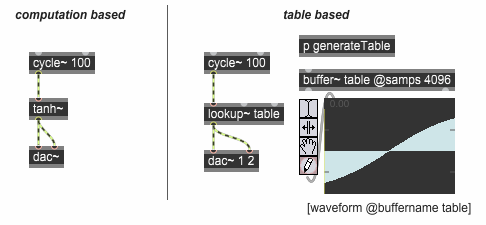
\includegraphics[width = 14cm]{tableVsCPU.png}
		\caption{Left: using a mathematical function to calculate the output. Right: using a table to look up the output.}
		\label{fig:tableVsCPU}
	\end{center}
\end{figure}





\subsection{How is Waveshaping related to other techniques?}
\subsubsection{Sampling}
If we take a look at figure \ref{fig:RamFilePlayback}, we see that we play a sound file by accessing a buffer (wavetable) using an index, an oscillator. This is effectively the same setup as we would build for distorting an input sound. Also take a look at figure \ref{fig:identity}, which showing us that waveshaping and wavetable synthesis are identical.

\begin{figure}[H]
	\centering
	\includegraphics[width=11cm]{identityWaveshaping.png}
	\caption[farnell waveshaping identity]
	{Picture taken from \cite{farnell_designing_2010}, showing the identity of waveshaping and wavetable synthesis}
	\label{fig:identity}
\end{figure}



\subsubsection{Modulation}
While we will talk about modulation in a separate chapter, let's loosely define amplitude modulation (AM) as the multiplication of two oscillators and frequency modulation (FM) as varying the frequency of an oscillator using another oscillator.\
So, as we have also seen above, AM looks like this:
\begin{equation}
	y = sin(a)\cdot sin(b)
\end{equation}

and FM looks like this:

\begin{equation}
	y = sin(sin(a))
\end{equation}

in practice, the a and b terms are a bit more complicated, but we will look at this later. That certain cases of AM are identical to waveshaping has been shown above, think about the square function again.
This of course does not mean that waveshaping can do everything AM can do and it does not mean that AM can achieve everything that waveshaping can. This should just show that we can understand the techniques from the perspective of another.\
What about FM? Well if our lookup function we use for waveshaping is a sine wave, we arrive at the exact same equation as how we defined FM above. Again, practically speaking, the results we get with these two techniques are very different, but we can see the connections.


\subsection{Why is Waveshaping useful?}
The output spectrum is dependent on the input amplitude. This makes it easy to create complex evolving spectra.

\subsection{What are the problems with waveshaping?}

Waveshaping adds overtones. When we build a waveshaper, we have to be aware of aliasing. Take a look at figures ~\ref{fig:clipped1} and ~\ref{fig:clipped2}. Sinewaves have been amplified and clipped here.

\begin{figure}[h!]
	\centering
	\includegraphics[width=11cm]{clippedSine.png}
	\caption[clipped sine wave]
	{A sine wave was generated and clipped. Clipping is a form of waveshaping which adds many overtones. Note how high frequencies fold back into the lower parts of the spectrum because they exceed the Nyquist-rate.}
	\label{fig:clipped1}
\end{figure}

\begin{figure}[h!]
	\centering
	\includegraphics[width=11cm]{clippedSine2.png}
	\caption[clipped sine wave 2]
	{Again, a sine wave, this time with a higher frequency to begin with. Extreme clipping has been applied by boosting the input amplitude. The aliased overtones are all over the place, even below the input frequency.}
	\label{fig:clipped2}
\end{figure}

In pd we could achieve this like in figure \ref{fig:pdClipping}.

\begin{figure}[H]
	\begin{center}
		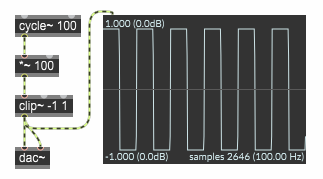
\includegraphics[width = 4cm]{img/pdSineClipping.png}
		\caption{Clipping an amplified sine wave in pd}
		\label{fig:pdClipping}
	\end{center}
\end{figure}

What does the output look like? Let's not only look at the spectra but also at the time signal:


\begin{figure}[H]
	\begin{center}
		\includegraphics[width = 14cm]{sineClipTime.png}
		\caption{An amplified and clipped sine wave in the time domain.}
		\label{fig:timeClip}
	\end{center}
\end{figure}

We see that we can arrive at a square-wave like result, but this square-wave is not anti-aliased.\\

The problem of aliasing in waveshaping is usually treated by over-sampling. This does not solve the problem but lessens it significantly resulting in cleaner, arguably better sound. Oversampling means that, if we work at a sample-rate of 44.1kHz, the input is up-sampled, essentially interpolated, to be at a sample-rate of 88.2kHz. Then the waveshaping is applied, leaving room for high frequencies up to 44.1kHz. Using a lowpass filter, high frequencies over 22.1kHz are then attenuated as much as possible, in order to be able to down-sample again to reach our initial sample-rate of 44.1kHz. \\
To state it more simple: Waveshaping is usually encapsulated in a process that runs at higher sampling rates in order to lessen aliasing.


% Wieso ist waveshaping praktisch? Amplitudenabhängigkeit d. spectrums.
% Wieso ist waveshaping verwandt mit modulation, sowohl FM, PM als auch AM? Am: siehe \(x^2\). FM: siehe \(f(x)=cos(x)\). Auch kann letztendlich eine transferkuntion in cos/sin bestandteile zerlegt werden um zu einer menge an frequenzmodulationen anzukommen, bzw kann der wavetable als polynom angenähert(o. Taylor entwicklung) werden um bei AM anzukommen.



\section{Sampler}
In pure data (but also in general) we can choose to play a sound from RAM or more or less\footnote{the data played from disk needs to be cached also} directly from the hard disk. Both Approaches have their different use-cases.\\


\video{In video, we need to make the same decision essentially. We can choose to buffer as much as we can on the VRAM of the graphics card or rather play from disk. Also different codecs specialize on balancing the load differently. The HAP codec for example tries to only push as much of the load to the hard disk and as little as possible to the CPU (which is decoding the video for playback). In times of SSDs this is a very good (and scalable) method to push a lot of data to playback in realtime.}
\textit{Work in progress.}

\begin{figure}[H]
	\begin{center}
		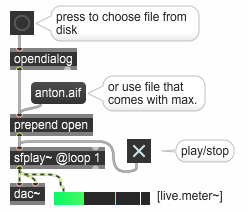
\includegraphics[scale = 1]{img/sampler.png}
		\caption{simpleSampler}
		\label{fig:simpleSampler}
	\end{center}
\end{figure}

\begin{figure}[H]
	\begin{center}
		\includegraphics[scale = 0.5]{img/soundFileToRam2.png}
		\caption{sound in Ram}
		\label{fig:soundRam}
	\end{center}
\end{figure}


\begin{figure}[H]
	\begin{center}
		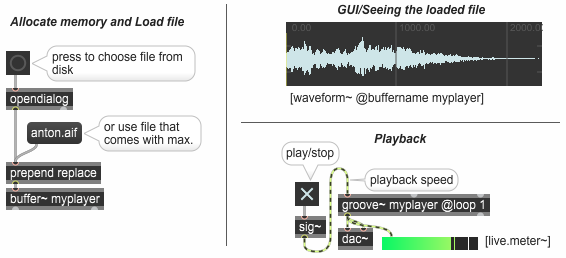
\includegraphics[scale = 1]{img/RamFilePlayback.png}
		\caption{RamFilePlayback}
		\label{fig:RamFilePlayback}
	\end{center}
\end{figure}



\begin{figure}[H]
	\begin{center}
		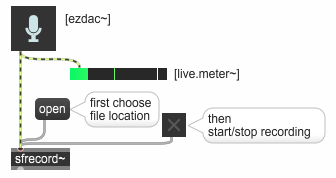
\includegraphics[width = 14cm]{writingAudio.png}
		\caption{writing Audio to disk}
		\label{fig:writing}
	\end{center}
\end{figure}

\bgInfo{
\subsection{Granular Sampling}
In figure \ref{fig:granular} you see the basic structure of granular sampling. Granular sampling allows us for example to playback a file slower without lowering the pitch. It is one of the methods to make speed and ppitch independent from each other during playback. Other methods also include FFT based approaches.

\begin{figure}[H]
	\begin{center}
		\includegraphics[width=\textwidth]{img/grain2.png}
		\caption {The patcher \href{./patchers/01\_waveshaping/granular.pd}{\texttt{patchers/01\_waveshaping/granular.pd}}, a simplified version of granular sampling}
		\label{fig:granular}
	\end{center}
\end{figure}
}


\section{Key Points}

\begin{itemize}
	\item When do we sampling from RAM when from disk?
	\item what are the problems with waveshaping?
	\item Make sure you understand that waveshaping can produce overtones.
	\item Make sure if you see a (simple) mathematical expression you can decide if it is non-linear or not.
	\item Make sure you recognize waveshaping in pd if you see it (e.g. figure \ref{fig:squarePd} )
\end{itemize}


% \section{Hausübung}
% \subsection{Testmodul}

% baue ein audio Testmodul mit folgener spezifikation:\\
% \begin{itemize}
% 	\item Ein audio output
% 	\item verschiedene klangquellen wählbar:
% 		\begin{enumerate}
% 			\item White Noise
% 			\item Sinus (freq. einstellbar)
% 			\item soundfile (file wählbar)
% 		\end{enumerate}
% 	\item GUI
% 	\item verfügbar(in eurem pfad, und jederzeit abrufbar als abstraction)
% 	\item output pegel sichtbar (level meter)
% \end{itemize}


% \begin{figure}[H]
% 	\begin{center}
% 		\includegraphics[scale = 1]{img/audioTester.png}
% 		\caption{audioTester.pd, zu bauen als Hausübung}
% 		\label{fig:audiotester}
% 	\end{center}
% \end{figure}

%!TEX root = main.tex

\chapter{Modulation}
\label{chap:modulation}


\begin{figure}[H]
	\begin{center}
		\includegraphics[width = 14cm]{img/surface-modulation_3.jpg}
		\caption{``Surface Modulation'' by Richard Sweeney}
		\label{fig:Surface Modulation}
	\end{center}
\end{figure}


\begin{center}
\begin{figure}[h!]
\tikzset{concept/.append style={fill={none}}}
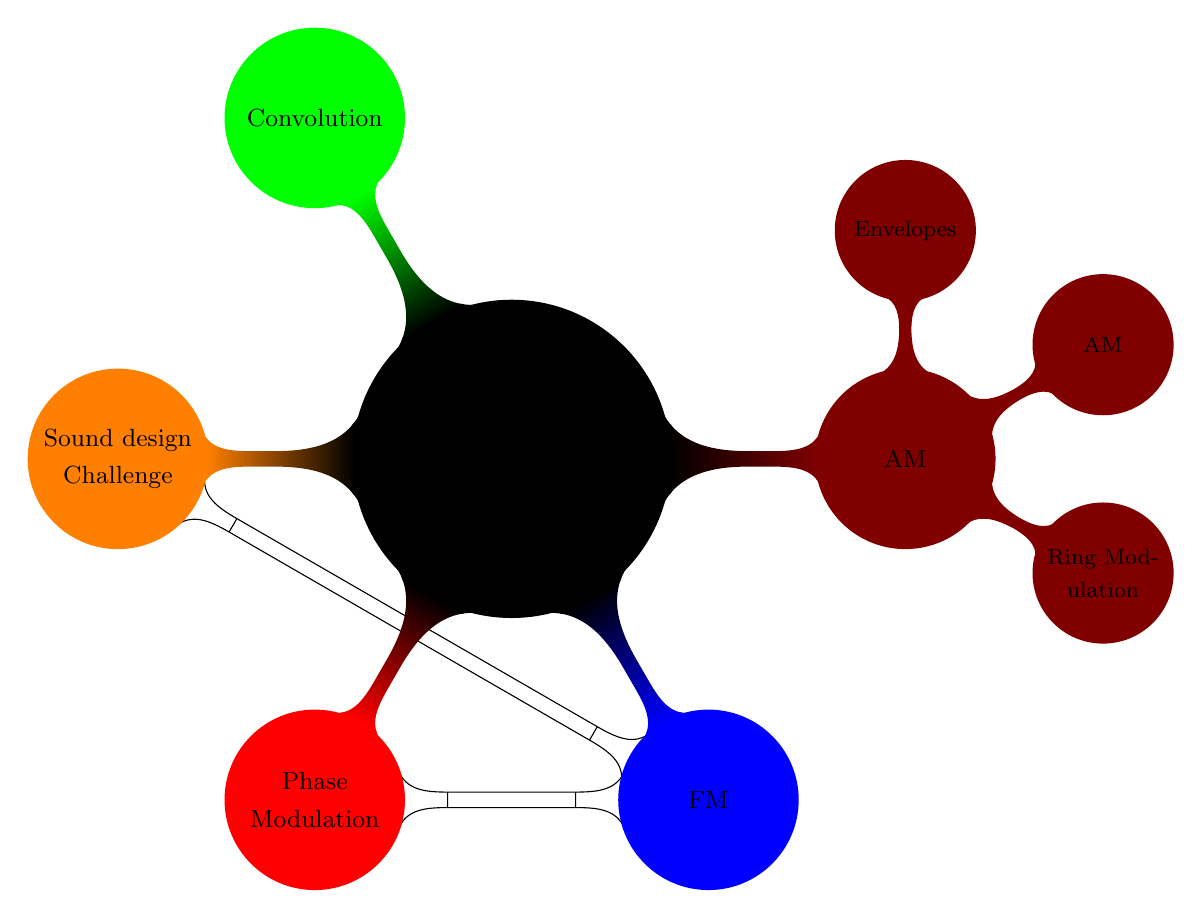
\begin{tikzpicture}
  \path[mindmap,concept color=black,text=black]
    node[concept] {Modulation}
    [clockwise from=0]
    child[concept color=red!50!black] {
      node[concept] {AM}
      % }
      [clockwise from=90]
      child { node[concept] {Envelopes} }
      child { node[concept] {AM} }
      child { node[concept] {Ring Modulation} }
      % child { node[concept] {pro\-gramming languages} }
      % child { node[concept] {software engineer\-ing} }
    }
    child[concept color=blue] {
      node[concept] (fm) {FM}
      [clockwise from=-30]
    }
    child[concept color=red] { node[concept] (pm){Phase Modulation} }
    child[concept color=orange] { node[concept] (sd) {Sound design Challenge} }
    child[concept color=green] { node[concept] (conv) {Convolution} };


\begin{pgfonlayer}{background}
    \draw [circle connection bar]
      (fm) edge (sd)
      (fm) edge (pm);
  \end{pgfonlayer}

\end{tikzpicture}
\caption{Lecture Contents}
\end{figure}
\end{center}


% \section{Notizen}

% kürzer. Modulation als sub einheit einplanen.
% Sounddesign challg. halbe stunde ok..

% Passt garnicht: (weil eher additive synth)
% https://www.youtube.com/watch?v=oKv9S6mxnXE

% Convolution anreissen?
% Notation durchgehen.

% Aliasing besprochen?
% \href{https://www.youtube.com/watch?v=GBtHeR-hY9Y}{Water experiment}
% (youtube \glqq{}The Secret to Levitation\grqq{})

% AM, tremolo

% Envelopes in pd

% FM, vibrato

% sounddesign chall.

% Hü

\section{Convolution}
\label{sub:conv}
Before talking about modulation, we should quickly look at what's convolution\footnote{'Faltung' in German}.\\
Convolution is a mathematical operation, widely used in signal processing but also in other fields. Convolution of two functions, say, $x$ and $h$ is typically denoted as $x*h$. \textbf{Note that $*$ does not mean multiplication here, it means convolving $x$ with $h$}. Obviously this can lead to confusion in some cases, but notation problems are not uncommon in sciences.\footnote{e.g while mathematicians use $i$ as the imaginary number, electrical engineering folks use $j$ (their $i$ is electrical current.).}\\

We will define Convolution of a function $x$ with a convolution kernel $h$ of length $N$as\footnote{You will find different definitions online. The given definition seems more intuitive but is not very common. Here is a common one:$y(n) = \sum_{k=-\infty}^{\infty} x(k) h (n-k)$}:

\begin{equation}
y(n) = \sum_{k=0}^{N-1} x(n-k) h (k)
\end{equation}
In words: for every output sample $y(n)$ take the current input sample $x(n)$ times the first sample of the convolution Kernel $h(0)$ plus take the previous input sample $x(n-1)$ times the second sample of the convolution kernel $h(1)$ plus the third last input sample $x(n-2)$ times the third sample of the convolution kernel $h(2)$ and so on... until the $Nth$ sample of $h$. It can be viewed as a a weighted average of the previous input samples, with weighting coefficients found in $h$.

We will look at convolution in a later chapter. If you  are eager to know more about convolution can have a look at
\href{https://youtu.be/_vyke3vF4Nk?t=25m14s}{this}\footnote{https://youtu.be/\_vyke3vF4Nk?t=25m14s}. \link{http://www.songho.ca/dsp/convolution/convolution2d\_example.html}{Here} is an example of convolution in 2D. Convolution in 2D is actually a bit easier to understand and is usually done to achieve a blur effect on an image or video. But why mention convolution if it is not explained at this point? Amplitude modulation and convolution just have a very close relationship, an that is:
\important{Multiplying two signals in the time domain is equivalent to convolution in the frequency domain and convolution in the time domain is equivalent to multiplication in the frequency domain.
}



\section{AM} % (fold)
\label{sub:AM}
In this section we will try amplitude modulation. Amplitude modulation is used for radio communication (so you'll need to understand this as a technician, modulation techniques are extremely important and this is maybe the simplest one) but also in sound design. We will try to understand the problem from different perspectives at once:
\begin{itemize}
	\item Doing some math
	\item listening to it
	\item brining it in context to beating waves
	\item seeing it as convolution in the frequency domain
\end{itemize}

Amplitude modulation means modulating the amplitude of a signal(surprise!). Modulating means changing over time by another signal. So we have some signal, say, a sine wave, and change its amplitude with another signal, say, another sine wave. Taking this concept and reducing it radically, we end up with figure \ref{fig:simpleAM}.

\begin{figure}[H]
	\begin{center}
		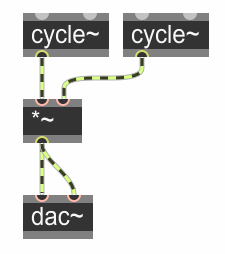
\includegraphics{img/ringNaive.png}
		\caption{Simplest form of ``Ring modulation''.}
		\label{fig:simpleAM}
	\end{center}
\end{figure}
Of course, we get no sound in figure \ref{fig:simpleAM} because the frequencies are not initialized, but it shows the general principle. The caption of that figure says ``Ring Modulation''. Let's quickly get some vocabulary straight:\\
\begin{itemize}
	\item ``Amplitude modulation'' might mean any modulation of amplitude
	\item ``Ring Modulation'' means \textit{bi-polar} amplitude modulation.
	\item In sound design, ``Amplitude Modulation'' might specifically mean unipolar amplitude modulation.
\end{itemize}

And some more vocabulary to put what we are doing in a musical context:
\begin{itemize}
	\item Modulating the amplitude is called ``Tremolo'' in music \footnote{sadly, the fender Stratocaster's ``Tremolo Arm'' is used to control the pitch. Ignore Fender, they got it wrong. You can trust that most guitar players are confused because of this.}
	\item Modulating the pitch or frequency (``FM'') is called ``vibrato'' in a musical context.\footnote{Maybe think about it like this: The F in FM is a bit like the v in vibrato. Just to avoid confusion..}
\end{itemize}

Enough words, let's look at what AM looks like, look at figure \ref{fig:AMViz}.

\begin{figure}[h!]
	\centering
	\includegraphics[width=\textwidth]{AMviz.png}
	\caption[AM time domain]
	{Looking at AM in the time domain}
	\label{fig:AMViz}
\end{figure}

\begin{question}
	If we would listen to the signal depicted in the bottom plot of figure \ref{fig:AMViz}, what do you think we would hear? Try to imagine! If you can't, use pure data to test it! That's why we are using pd.
\end{question}
\begin{Answer}
	We would hear a 30Hz sine wave repeatedly rising and falling in amplitude.
\end{Answer}

\begin{question}
	Next question, same plot, same signal. So hopefully you found out that we hear a 30 Hz sine with rising and falling amplitude. At what frequency does the amplitude rise and fall? Remember we are modulating with a 1 Hz sine.
\end{question}
\begin{Answer}
	Two Hertz.
\end{Answer}

You can try out plotting what happens with different frequency settings in \link{https://colab.research.google.com/drive/1oO3ApcIfvcUoIqv9\_nDS-HNl8B4Gf5hl}{this Notebook}.

Maybe you remember from the waveshaping chapter that we actually calculated what frequencies should come out of AM. Also maybe you remember that:

\important{
Amplitude Modulation produces sum and difference frequencies of the input frequencies.
\begin{equation}
	cos(a)\cdot cos(b) = \frac{cos(a+b) + cos(a-b)}{2}
\end{equation}
}
But here we still hear the 30 Hz, just getting louder and softer, so what's wrong?\\
So, let's calculate this. We have two oscillators, $x_1(t) = cos(30t2\pi)$ and $x_2(t)=cos(t2\pi)$. We multiply them, ending up with:

\begin{equation}
	y(t) = cos(30t2\pi) \cdot cos(t2\pi)
\end{equation}
Ok, the above formula tells us this means:
\begin{equation}
	y(t) = \frac{cos(30t2\pi+t2\pi)+cos(30t2\pi-t2\pi)}{2}
\end{equation}
We can now simplify to:
\begin{equation}
	y(t) = \frac{cos((30+1)t2\pi)+cos((30-1)t2\pi)}{2} = \frac{cos(31t2\pi)+cos(29t2\pi)}{2}
\end{equation}

Hm, so we get out a 31Hz and 29Hz oscillator. What about that rising and falling in amplitude that we hear \textit{and} observe in the plot, surely there must be something wrong! Do you have a solution to this?\\

Let's use pure data to help us understand. Make two oscillators, one with 29Hz and one with 31Hz, what do you hear?

\begin{figure}[h!]
	\centering
	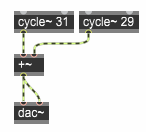
\includegraphics{beating.png}
	\caption[adding two oscillators]
	{Adding two oscillators with frequencies very close to each other}
	\label{fig:beating}
\end{figure}

If you listen to what is depicted in figure \ref{fig:beating}, you will in fact hear the same as if you do the 30Hz /1 Hz amplitude modulation (which indicates that our formula above is correct). What we hear is a phenomenon called beating(``Schwebung''). The phase of the two oscillators is canceling each other out at regular intervals because the frequencies are so close to each other. In fact the frequency of the beating $f_{beat}$ is always
\begin{equation}
	f{beat}=|f_1-f_2|
\end{equation}
So the difference of the two frequencies.


% \comm{vline and envelop description missing}
% \begin{figure}[H]
% 	\begin{center}
% 		\includegraphics[width = 14cm]{img/simpleEnv.png}
% 		\caption{caption}
% 		\label{fig:name}
% 	\end{center}
% \end{figure}

\section{FM} % (fold)
\label{sub:FM}

Frequency modulation can be used to modulate the frequency, meaning to vary the pitch of a sound, see figure \ref{fig:fmSlow}. But it can also be used to generate overtones and an overall richer spectrum, see figure \ref{fig:fmFast}. The two ``different versions'' only differ from each other by different parameter\footnote{We see which parameters can be adjusted in a minute. But if you want to know them now: modulation frequency, modulation amount and carrier frequency.} values being used.
We can think of Frequency Modulation (FM) as something of the form:

\begin{equation}
	y(t) = cos(cos(b))
\end{equation}

This really is a simplification, but the overall structure of the formula is correct.
% FM is mathematically very similar to phase modulation.
Looking at figure \ref{fig:fmIdea} we can see the very basic idea implemented in pure data.
\begin{figure}[H]
	\begin{center}
		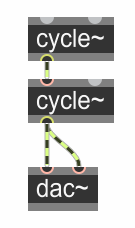
\includegraphics{img/FMgeneral.png}
		\caption{The General Idea of FM}
		\label{fig:fmIdea}
	\end{center}
\end{figure}

Since the frequencies of the oscillators are not set, we won't hear anything when building this patcher. But looking at it may reveal that the idea simply is to control the frequency of an oscillator using another oscillator.\\
We can expand the patcher by adding some math to make it more usable, as in figure \ref{fig:fmNaive}.

Naive parameters are ${f_c}$ (Carrier Frequency), ${f_m}$ (Modulator Frequency), and ${A_m}$ (modulation Amount).

\begin{figure}[H]
	\begin{center}
		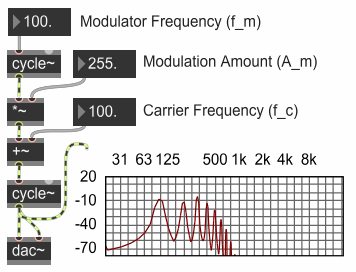
\includegraphics{img/FMnaive.png}
		\caption{Naive Implementation with Direct Parametrization.}
		\label{fig:fmNaive}
	\end{center}
\end{figure}

\important{

The output frequencies will be
\begin{equation}
	f_c \pm n \cdot f_m
\end{equation}

for $n$ being all integers. So the carrier frequency plus and minus integer multiples of the modulation frequency. We get many (theoretically infinitely) many overtones with different amplitudes this way.
}
\bgInfo{
	The amplitudes of the different frequencies are determined by Bessel functions which makes it so seemingly random.
		\centering
		\includegraphics[width=11cm]{bessel}
}


Typically, FM is controlled via \textit{Index}, \textit{Ratio}, and fundamental Frequency.
The Index, ${I}$ is given by Modulation Depth and Modulator Frequency.


% =============Something is wrong with this.============================

% \begin{mdframed}[backgroundcolor=black!10,rightline=false,leftline=false]
\bgInfo{
\begin{equation}
I = \frac{A_m}{f_m} % verified via http://computermusicresource.com/FM.synthesis.html
\end{equation}

A more controllable Implementation will generate the naive parameters from a Ratio, ${R}$, the Carrier Frequency and the Index:
\begin{equation}
	f_m = \frac{f_c}{R}
\end{equation}

\begin{equation}
	A_m = I \cdot f_m
\end{equation}

\begin{figure}[H]
	\begin{center}
		\includegraphics{img/FMcorrect.png}
		\caption{FM with Index and Ratio}
		\label{fig:fmComplete}
	\end{center}
\end{figure}

But there are also different implementations such as:
\begin{figure}[H]
	\centering
	\includegraphics[width=5cm]{fmMillerPuckette}
	\caption[miller Puckette FM]
	{Fm implementation from \cite{miller_puckette_theory_2006}}
	\label{fig:label}
\end{figure}

% ===========FIND EN EXPLANATION FOR THE ABOVE FM implementations=============


% \end{mdframed}
% =========================================================================
}

\begin{figure}[h!]
	\centering
	\includegraphics[width=\textwidth]{FMslow}
	\caption[FM visualization, low freq]
	{Modulator frequency: 1Hz, Crarrier Frequency 50 Hz, Modulation Amount 10. Please ignore the labeling of the Y axis of the spectrum plot($10^0$). It is wrong. The y axis goes from 0 to nyquist=22050Hz.}
	\label{fig:fmSlow}
\end{figure}


\begin{figure}[H]
	\centering
	\includegraphics[width=\textwidth]{FMfast}
	\caption[FM visualization, hi freq]
	{Modulator frequency: 100Hz, Crarrier Frequency 1000 Hz, Modulation Amount 0.5. Please ignore the labeling of the Y axis of the spectrum plot($10^0$). It is wrong. The y axis goes from 0 to nyquist=22050Hz.}
	\label{fig:fmFast}
\end{figure}


\section{Key Points}
\begin{itemize}
	\item Make sure you understand the differences between AM and FM
	\item Make sure you recognize what form of modulation is present if you see a patcher or a simplfied formula (like: $sin(a) \cdot sin(b)$ what form of modulation is this?)
	\item make sure you could make such a simplified formula if you see a patch and vice versa.
	\item make sure you know what frequencies result from an amplitude modulation
	\item make sure you know what frequencies result from a frequency modulation
\end{itemize}

% \section{Hausübung}
% \label{sub:Hausuebung}
% Andy Farnell, \href{http://aspress.co.uk/ds/pdf/pd_intro.pdf}{pd intro} chapter 6, lesen

%!TEX root = main.tex
\chapter{Filters}
\label{chap:filters}


\begin{figure}[H]
	\begin{center}
		\includegraphics[width = 14cm]{img/Narciss_Caravaggio.jpg}
		\caption{Caravaggio, Narziss. ad Feedback: Echo liebt Narziss etc.}
		\label{fig:name}
	\end{center}
\end{figure}

\begin{center}
\begin{figure}[h!]
\tikzset{concept/.append style={fill={none}}}
\begin{tikzpicture}
  \path[mindmap,concept color=black,text=black]
    node[concept] {Filters}
    [clockwise from=0]
    child[concept color=red!50!black] {
      node[concept] {Systems}
      % }
      [clockwise from=90]
      child { node[concept] {Impulse Response} }
      child { node[concept] {Difference Equation} }
      child { node[concept] {Transfer Function} }
      % child { node[concept] {pro\-gramming languages} }
      % child { node[concept] {software engineer\-ing} }
    }
    child[concept color=blue] {
      node[concept] (IIR) {IIR}
      [clockwise from=-30]
    }
    child[concept color=red] { node[concept] (FIR){FIR} }
    child[concept color=orange] { node[concept] (sd) {Sound design Challenge} };


\begin{pgfonlayer}{background}
    \draw [circle connection bar]
      (fm) edge (sd)
      (fm) edge (pm);
  \end{pgfonlayer}

\end{tikzpicture}
\caption{Lecture Contents}
\end{figure}
\end{center}




What is a filter? We use filters a lot. We often need to shape the spectrum of a signal. Be it for technical reasons (DC-Offset removal, Anti-aliasing filters, crossovers, interpolation, ...) or for aesthetic ones (EQ-ing, subtractive synthesis)\\
Please take a moment and seriously ask yourself, knowing what you know about signals, knowing what we can do with a computer: How do we actually do this? What is a digital Filter? This is what this chapter will try to explain.\\

\section{Seeing Frequency Content in the Time Domain}

Let's first try to get a feel for how signals \textit{look}. It's a lot easier to understand how a filter works afterwards. This might be obvious but let's state clearly:

\begin{framed}
	High frequency signals have a short \textit{period}. That means the signal ``moves'' fast, or a lot in short time. Therefore: The more movement is in a signal or the more fluctuation or the faster the signal changes the more high frequency content it has.
\end{framed}


Three Questions in order to make you think about signals:


\begin{question}
	Please look at the image below. Can you draw an approximation of its spectrum? What signals could have been mixed to obtain this result? To help you think about this: How would you explain the graph to somebody who doesn't see it?
% subsection raetsel (end)
\begin{figure}[H]
	\begin{center}
		\includegraphics[width = 14cm]{raetsel_original.png}
		\caption{Original Signal}
		\label{fig:originalSignal}
	\end{center}
\end{figure}
\end{question}


\begin{Answer}
You should be able to see that there is a sinusoidal component in the signal. This sinusoid has a period of 10 ms, so a frequency of 100 Hz. But also you should see that it is not a clean sine wave, there is some noisy component in there. This is what you should have been able to infer from the image. In fact it is an (attenuated) 100Hz sinusoid mixed with (attenuated) white noise.
\end{Answer}


\begin{question}
	The signal in figure \ref{fig:originalSignal} was filtered. As a result we obtained the signal in figure \ref{fig:filtered1}. What kind of filter could have been used?
	\begin{figure}[H]
	\begin{center}
		\includegraphics[width = 14cm]{raetsel_highpass.png}
		\caption{Filtered Signal 1}
		\label{fig:filtered1}
	\end{center}
	\end{figure}
\end{question}

\begin{Answer}
	It could have been a notch or stopband filter at 100 Hz or a highpass. In fact, it was a highpass.
\end{Answer}


\begin{question}
	Again, the signal in figure \ref{fig:originalSignal} (so the original signal again) was filtered. As a result we obtained the signal in figure \ref{fig:raetsel_2} . What kind of filter could have been used?
\begin{figure}[H]
	\begin{center}
		\includegraphics[width = 14cm]{raetsel_lowpass.png}
		\caption{Filtered Signal 2}
		\label{fig:raetsel_2}
	\end{center}
\end{figure}

\end{question}


\begin{Answer}
	It could have been a bandpass at 100Hz, or a lowpass. In fact, it was a lowpass. We see that the signal got a lot smoother.
\end{Answer}

\section{Ways of Describing a Filter}
There are a couple of ways to \textit{fully} describe a linear time invariant system (LTI), filters typically\footnote{filters can be augmented with non-linear or time-varying elements, for example distortion or modulation. In sound design, this is actually very common. But describing such a system mathematically is out of the scope of this work.} are such systems.\\
Below is an (incomplete) list of methods that are all able to describe a filter. They offer very different possibilities of understanding and manipulating a filter.
\begin{itemize}
	\item Difference Equation
	\item Magnitude and Phase Response
	\item Impulse Response
	\item Code (graphical, such as pd)
	\item Code (text, such as C++)
	\item Block Diagram
	\item Transfer Function (Rational Function)
	\item Unit Step Response
\end{itemize}


\begin{figure}[htb]
  \centering
  \label{fig:string}

  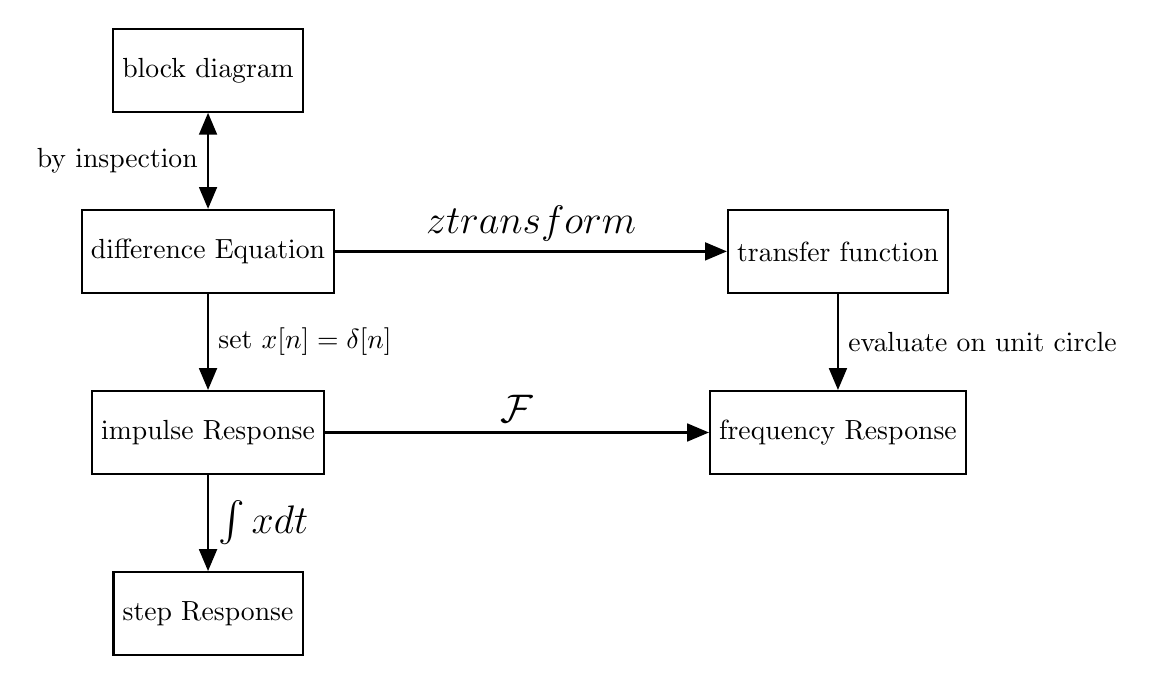
\begin{tikzpicture}[auto, thick, node distance=2.3cm, >=triangle 45]

  % \draw node at (0,0) [input] (excitation) {};
  \draw node at (0,0) [block] (de) {difference Equation};
  \draw node [block, right of=de, node distance = 8cm] (tf) {transfer function};
  \draw node [block, below of= de] (ir) {impulse Response};
  \draw node [block, below of= ir] (sr) {step Response};
  \draw node [block, below of= tf] (fr) {frequency Response};
  \draw node [block, above of= de] (bd) {block diagram};



  % \draw node [block, below of=delay, node distance = 2cm] (loss) {\Large$G(z)$};
  % \draw node at (6.,-0.001) {\textbullet};

  % \draw node [output, right of=delay,node distance = 3cm] (out) {};
  \draw[<->] (de) -- node {by inspection}(bd);
  \draw[->] (de) -- node {\Large$z transform$}(tf);
  \draw[->] (tf) -- node {evaluate on unit circle}(fr);
  \draw[->] (de) -- node {set $x[n]=\delta[n]$}(ir);
  % \draw[->] (sum1) -- node {}(delay);
  % \draw[->] (loss.west) -| node {}(sum1.south);

  % \draw[->] (6., -0.001) |- node {}(loss.east);


  \draw[->] (ir) -- node {\Large$\int x dt$}(sr);
  \draw[->] (ir) -- node {\Large$\mathcal{F} $}(fr);
  % \draw[<-] (ir) -- node {\Large$\mathcal{F^{-1}} $}(fr);

  \end{tikzpicture}
  \caption{Ways of describing LTI systems and how to get from one to the other}
\end{figure}




While in practice, the transfer function is very important, we will mostly work with block diagrams, pd programs and difference equations.\\
It is an important skill to be able to switch between these representations, for example to calculate the impulse response from a difference equation or block diagram.

\subsection{Difference Equations}
\label{sub:diff}

A difference equation is of the form mentioned in the introduction. So for example
\begin{equation}
	y(n) = x(n)+x(n-1)
	\label{eq:simple}
\end{equation}
Here, $y$ is the output $x$ is the input and $n$ denotes indexing those two signals.\\
$y(n)=x(n)$ means: take the incoming sample and make it the output. $x(n-1)$ denotes a delay by one sample. Please note that the above equation describes a \textit{system}, a filter in this case. But it can be seen as using an input array (the input signal), indexed by $n$ and creating an output array.\\
Let's visualize this idea. Given the input signal in figure \ref{fig:diffImpResp}, we can create the output using the equation.

\begin{figure}[h]
	\centering
	\includegraphics[width=\textwidth]{diffEqViz1}
	\caption[shortCaption]
	{The input and corresponding output of the equation given above.}
	\label{fig:diffImpResp}
\end{figure}
 Also it becomes obvious that the $n-1$ expression is a delay, since it makes us look up the 3rd index for creating the 4th sample at the output in this case, or $y(4) = x(4)+x(4-1)$.\footnote{The impulse in this example input signal is at position $n=3$ so the third sample. This was chosen at random and has no meaning. It could just as well sit at $n=5$.}\\
 So for more clarity, let's see all the values at all $n$s (compare this with figure \ref{fig:diffImpResp}):

\begin{center}

\begin{tabular}{l|l|l|l}
	$n$ & $y(n)$ & $x(n)$ &$x(n-1)$\\
	\hline
	0 & 0 & 0 &0\\
	1 & 0 & 0 &0\\
	2 & 0 & 0 &0\\
	3 & 1 & 1 &0\\
	4 & 1 & 0 &1\\
	5 & 0 & 0 &0\\
\end{tabular}
\end{center}



\subsection{Block Diagrams} % (fold)
\label{sub:block}

Block diagrams are nice because they are very visual and sometimes easier to understand. Also, if we work in pure data, or a different graphical programming language (such as Max/MSP or MATLAB Simulink) it's very straight forward to implement a block diagram. Translating from a block diagram to text code or difference equations or vice versa can be hard sometimes.\\
In figure \ref{fig:diffImpResp}, we can see a block diagram representation of equation \ref{eq:simple}. This \textit{is} the same thing.

% subsection subsection_name (end)

\begin{figure}[H]
  \centering
  \label{fig:string}
  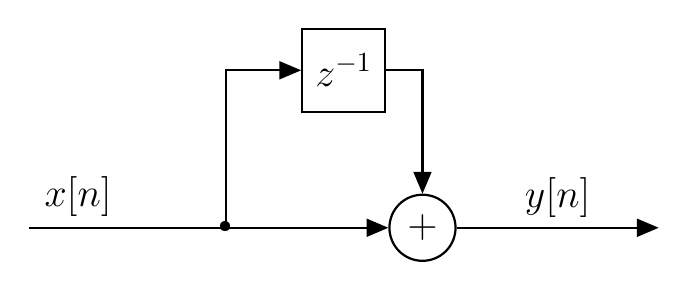
\begin{tikzpicture}[auto, thick, node distance=2.5cm, >=triangle 45]
  \draw node at (0,0) [input] (inp) {};
  \draw node at (2.5,-0.001) (junct) {\textbullet};
  \draw node at (4,2) [block] (delay) {\Large$z^{-1}$};
  \draw node [sum, right of=inp, node distance = 5.cm] (sum1) {\Large$+$};

  \draw node [output, right of=sum1,node distance = 3cm] (out) {};
  \draw[->] (inp) -- node {}(sum1);
  % \draw[->] (junct) |- node {}(delay);
  \draw[->] (delay.east) -| node {}(sum1.north);

  \draw[->] (2.5, -0.001) |- node {}(delay.west);


  \draw[->] (sum1) -- node {\Large$y[n]$}(out);

  \node[text width=3cm] at (1.7,0.4)
    {\Large$x[n]$};

  \end{tikzpicture}
  \caption{A very simple lowpass filter.}
  \label{fig:blockDiagr}
\end{figure}

Don't be irritated by the $z^{-1}$ block. This notation stands for a delay by one sample. A block $z^{-m}$ would stand for a delay by $m$ samples. This is a convention we need to remember. This way of notating a delay might seem unnecessarily complex, but it has its reasons.

\bgInfo{This notation, $z^{-1}$, comes from the fact that analyzing the frequency response of a system is very easy when working with complex numbers (so compounds of real and imaginary numbers). Complex numbers are often denoted by $Z$, which is another convention. Not only do we work with complex numbers, but with complex sinusoids when analyzing such systems. We imagine complex sinusoids coming into our system. A multiplication by another complex sinusoid can cause a phase shift (a delay). Dividing ($z^{-1} = \frac{1}{z}$) an incoming complex sinusoid by the complex sinusoid at the same frequency causes a phase shift that is equals to a delay by 1 sample. If you want to understand all this and stop with mickey-mouse-explanations I can recommend reading \cite{miller_puckette_theory_2006} and \cite{smith_introduction_2007}. Both of these works can be found on-line for free.\

But let's quickly calculate the frequency response, so you've seen it once:
We take our difference equation (we could also start from the block diagram):
\begin{equation}
	y(n) = x(n)+x(n-1)
\end{equation}
We then do a process called the z-transform, that is, we get rid of all the indexing. We now think about applying the process of filtering to the whole signal at once and we denote the delay by a multipliaction with a complex sinusoid that causes a phase shift:
\begin{equation}
	Y = X + X \cdot Z^{-1}
\end{equation}

We then solve the equation for $Y/X$:

\begin{equation}
	Y = X \cdot (1 + Z^{-1})
\end{equation}
\begin{equation}
	\frac{Y}{X} = 1+Z^{-1}
\end{equation}

Typically we substitute $\frac{Y}{X}$ with a new name, typically $H$ and now make this a function of $Z$.

\begin{equation}
	H(Z) = 1 + Z^{-1}
\end{equation}
This is called a system's transfer function. This is the actual standard for talking about systems. Typically we do two things with this, either, we draw a so called \textit{Pole-Zero-Plot}.
\begin{figure}[H]
	\centering
	\includegraphics[width=\textwidth]{poleZero.png}
	\caption[pole zero plot]
	{a pole zero plot. This indicates where the function $H(z)$ has zeros(where its value is zero) or poles(where its value is infinity). Actually there is also a pole at $0+0i$ which is not shown here. This is because a pole at this position has no frequency dependent effect.}
	\label{fig:label}
\end{figure}

We can also evaluate the function $H(z)$for complex sinusoids.\\
The absolute value of $H$ is the output amplitude, if we just plot this value for all complex numbers we see this:

\begin{figure}[H]
	\centering
	\includegraphics[width=\textwidth]{poleZero3dPlot.png}
	\caption[poles and zeros, 3D in the complex plane]
	{Evaluation of the Transfer function in the complex plane. The unit circle is visible as a dotted line. This plot is not too easy to read but if you look at the coordinate $-1+0i$, you can see that the value there is very low. This seems to indicate a lowpass. You can basically ignore the huge mountain in the middle. It sits at $0+0i$ and has therefore equal effect on all frequencies.}
	\label{fig:label}
\end{figure}

It's OK if this plot doesn't tell you much. The really important thing is to evaluate this surface using complex sinusoids:
$cos(\omega) + i\cdot sin(\omega)$. This is the same as looking at the values along the dotted line. We can now plot the magnitude response over $\omega$. So we effectively evaluate the formula
\begin{equation}
	|H(\omega)| = |1 + (cos(\omega)+i \cdot sin(\omega))^{-1}|
\end{equation}
Where $\omega$ ranges from $0$ to $\pi$(sic!). This is the same as going along the dotted line, starting at $1+0i$ (lowest frequency) and ending at $-1+0i$ (the highest frequency). Then we finally get the magnitude response:

\begin{figure}[H]
	\centering
	\includegraphics[width=\textwidth]{magResp.png}
	\caption[Filter magnitude response]
	{Magnitude response, so $|H(\omega)| = |1 + (cos(\omega)+i \cdot sin(\omega))^{-1}|$}
	\label{fig:label}
\end{figure}



}

\subsection{pd Code} % (fold)
\label{sub:pd_code}
If we program the filter in pd (or any other programming language) we obviously also fully defined the filter. Try to build the filter from above in pd! Start from the difference equation or the block diagram, what ever is harder to understand for you.\\
In figure \ref{fig:pdSimpleFir} you can see the translation to pd.

\begin{figure}[H]
	\centering
	\includegraphics[width=5cm]{simpleFir}
	\caption[FIR filter in pd]
	{A simple filter in pure data.}
	\label{fig:pdSimpleFir}
\end{figure}



% subsection pd_code (end)

\subsection{Impulse Response}

An impulse has the advantage that it contains all frequencies. It has a flat spectrum.  So recording how a filter reacts to the impulse gives us the magnitude of the spectrum at all frequencies.\\
We can see the impulse response of the filter we are describing in this section in  multiple ways in figure \ref{fig:diffImpResp}.

\bgInfo{
\subsection{Text Oriented Code} % (fold)
\label{sub:tcode}
Below, we can see a code implementation in the language MATLAB.

\lstinputlisting[label=code,
captionpos=b,
caption=A script that creates an impulse implements a vectorized filter and plots the result.]{code/FIRvectorized.m}
}

\section{Ways of Getting an Intuitive Understanding}

So now we learned some ways to define a filter, to talk about a filter. But what is this filter actually doing? It is a very simple lowpass filter. It cuts away high frequencies. But why is adding a signal to itself but one sample delayed making a lowpass? This certainly is a bit surprising, so let's try to understand what's happening.

\subsection{Combfilter to Lowpass}
First let's view the problem from another angle. We know what this structure from above is: It's a combfilter, right? It's taking a signal and adding a delayed version of it. Let's quickly review what a combfilter is:
The combfilter effect can come up if we record something with a microphone and we get the direct signal and a delayed (e.g. via a reflection) signal also. These two signals mix together and this is what we get in our recording.\\
The result is that some frequencies cancel out.\\
We can simply simulate this situation in pd using a delay and an addition.

\begin{figure}[H]
	\centering
	\includegraphics[width=11cm]{simpleComb}
	\caption[simple comb filter]
	{A very simple comb filter}
	\label{fig:label}
\end{figure}

This canceling out of frequencies \footnote{also called destructive interference} can be imagined if we look at figure \ref{fig:destIntereference}.
\begin{figure}[H]
	\centering
	\includegraphics[width=\textwidth]{destInterference}
	\caption[Destructive Interference]
	{Destructive Interference. The two waves would cancel out completely if mixed together(=added).}
	\label{fig:destIntereference}
\end{figure}

Please note that the signal is a sine wave with a frequency of 100 Hz, so a period of 10 milliseconds. The delay is set to be 5 ms, so half of the period of the input signal in this case. It it was set to be equals the period, the two waves would \textit{interfere constructively}, so we would get out a higher amplitude. \\

\important{In a combfilter, the first frequency that cancels out is the one whose period is double the delay time. Or, to put it differently
\begin{equation}
	f_c = \frac{1}{2d}
\end{equation}
If $f_c$ is the first frequency that cancels out and d is the delay time in seconds. \\
How to calculate this fast, if you are given the delay time:
just calculate the frequency for the given delay, and then use half of that. For example, if given delay 1ms, the corresponding frequency would be 1000 Hz. Half of that (=double the period) is 500 Hz, and that's where the first trough in the spectrum would be.

}

In figure \ref{fig:combToLowpass} we can see the \textit{frequency response}\footnote{The impulse response is recorded a couple of times and the output's spectrum has been analyzed} of our combfilter. We see a couple of plots, it's always the same filter but the delay is different. We see that for delay times >1 sample, we observe our typical comb pattern. But at Delay = 1 sample, there is just a ramp left, leaving us with a lowpass.

\begin{figure}[H]
	\centering
	\includegraphics[width=\textwidth]{FromCombfilterToLowpass}
	\caption[From comb filter to lowpass]
	{Different amounts of delays result in different magnitude responses. The extreme case of a comb filter, a delay of 1 sample, is looking like a lowpass.}
	\label{fig:combToLowpass}
\end{figure}

\bgInfo{
	We can also calculate what's happening with our equation from above:
	The delay is $1/f_s$, so 1 over samplerate. This is called the sampling intervall, let's call it $I_s$, just to get rid of the fraction. The frequency that cancels out is then $1/2I$. By inspection we find that this means the frequency that has double the wavelength of the sampling frequency, so half the sampling frequency, so \textit{Nyquist}.
}


\subsection{Prolonging an Impulse}
We can also take a different route to understand why this is a lowpass. Let's recall what the spectrum of an impulse looks like and what the spectrum of DC offset looks like. Taking a look at figure \ref{fig:impToDc}, we see an impulse, the impulse response of our filter and a DC-Offset signal. Recalling from the introduction, and looking at the figure, we know that the DC-offset signal contains only energy at 0Hz. Now look at the time domain signals: Isn't making our impulse signal last for one sample longer a small step towards generating a DC-offset signal?

\begin{figure}[H]
	\centering
	\includegraphics[width=\textwidth]{impulseToDC}
	\caption[Spectrum Impulse, Lowpass, DC]
	{Impulse, impulse response and DC offset signal and their spectra. Note that there are very few samples here and the DC-Offset signal's spectrum seems to ramp down from 0Hz. In fact, there is a single high value at 0Hz.}
	\label{fig:impToDc}
\end{figure}

\subsection{A moving Average}
How is \textit{average} defined? There are a lot of different ways to compute an average, but typically we mean the \textit{arithmetic mean}, so adding all numbers and dividing by the count of items:
\begin{equation}
	A = \frac{1}{N} \sum_{n=1}^N x(n)
\end{equation}

Looking back at our filter, we will notice that we are adding up the current sample and the last sample. If we were to divide that sum by two (so the number of elements, since it's two samples we are adding up), we would arrive at the definition above. So we could say, that our lowpass is always outputting the average of the current and the last sample. It is therefore called a moving average filter. \\
Taking the average of something always reduces information and we get something that is fluctuating less than its input. If we would make a website or something that would always show the average temperature in Vienna of the last two weeks, this display wouldn't start jumping around if there was a single hot day in winter. It would remove high frequency data (jumps). It would be some kind of lowpass filter.


\subsection{A sine at Nyquist}
Here is yet another way of understanding why the structure we saw is a lowpass. Let's imagine a sine wave at Nyquist frequency, the highest frequency we can work with. We can see what such a sine looks like in Figure~\ref{fig:nyqSine}. If we apply this moving average filter, so that lowpass we have been talking about, what do you think comes out? Go ahead and calculate the average for each sample and its previous sample. We add $1 + -1 = 0$, $-1 + 1 = 0$, $1 + -1 = 0$, ... So you can see, if we feed a sine at nyquist into our lowpass, what we get is silence.


\begin{figure}[H]
	\centering
	\includegraphics[width=\textwidth]{sineWaveNyq.png}
	\caption[Sine wave at nyquist frequency]
	{Sine wave at nyquist frequency}
	\label{fig:nyqSine}
\end{figure}


\subsection{Highpass} % (fold)
\label{sub:Highpass}

You should already be familiar with the basic types of filters, so lowpass, highpass, bandpass etc. We now saw how we can build a lowpass filter, but what about a highpass, what about notching, peak, shelving filters? This is getting pretty involved quickly, but let's have a look at a highpass. Highpass filtering is the opposite of lowpass filtering. It emphasizes movement in the signal, since everything that moves fast must contain high frequencies. One simple form of a highpass is taking the difference between the current and the last sample, so:


\begin{figure}[H]
  \centering
  \label{fig:string}
  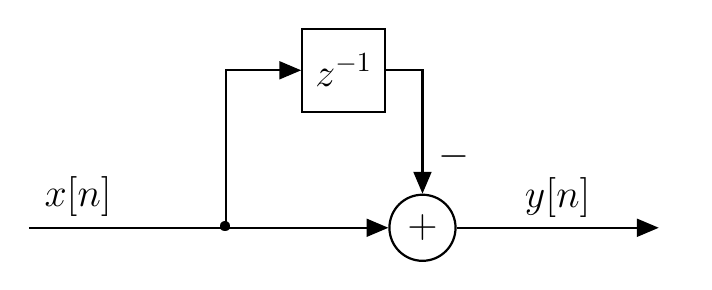
\begin{tikzpicture}[auto, thick, node distance=2.5cm, >=triangle 45]
  \draw node at (0,0) [input] (inp) {};
  \draw node at (2.5,-0.001) (junct) {\textbullet};
  \draw node at (4,2) [block] (delay) {\Large$z^{-1}$};
  \draw node [sum, right of=inp, node distance = 5.cm] (sum1) {\Large$+$};

  \draw node [output, right of=sum1,node distance = 3cm] (out) {};
  \draw[->] (inp) -- node {}(sum1);
  % \draw[->] (junct) |- node {}(delay);
  \draw[->] (delay.east) -| node {}(sum1.north);

  \draw[->] (2.5, -0.001) |- node {}(delay.west);


  \draw[->] (sum1) -- node {\Large$y[n]$}(out);

  \node[text width=3cm] at (1.7,0.4)
    {\Large$x[n]$};

\node[text width=3cm] at (6.7,0.9)
    {\Large$-$};


  \end{tikzpicture}
  \caption{A very simple highpass filter. Please compare to \ref{fig:blockDiagr}. }
  \label{fig:blockDiagrHigh}
\end{figure}

You will notice that figure \ref{fig:blockDiagrHigh} and figure \ref{fig:blockDiagr} are identical with oly one little exception. In this highpass filter we \textbf{subtract} the delayed signal from the input. This is denoted by the little $-$ sign next to one line leading to the addition. One might think, ``Why don't we just use a minus sign instead of the addition sign?'' Because order matters with subtraction, it makes a difference if we subtract 3 from 5 or 5 from 3.\\
The structure above is also called a differentiator, since it is a way of approximating the derivative of a signal.




% subsection filter_types (end)

\subsection{Video Filters}

\video{
	Filters in video work the same way and are as common as in audio. But in video we have another question to answer before we start filtering: Does our operation (adding two neighboring samples) apply to time, or to space? In other words: Do we want to add neighboring pixels to produce an output pixel or do we want to add whole frames over time to produce an output frame?\\
	Have a look at figure \ref{fig:v_origianl}. We will take this still from a video as a reference. We send the video through a couple of filters (one at a time, not in series) and watch the output. \\
	For each of the output frames, try to think about how this could have been generated from the input, what kind of a filter could have been used!?

	\begin{figure}[H]
		\begin{center}
			\includegraphics[width = 14cm]{vidFilters_o.png}
			\caption[Video Filters: Original]{Frame from the original video}
			\label{fig:v_origianl}
		\end{center}
	\end{figure}

\begin{figure}[H]
	\begin{center}
		\includegraphics[width = 14cm]{vidFiltersFIRs.png}
		\caption[Video Filters: Blur]{This effect is known as a \textit{blur} It is generalted by using a FIR lowpass in the space domain. That means, in the simplest case, each output pixel is the average of the input pixel at the same location and its neighbors. In practice, weighting functions are used to control, how much the input pixel and how much its neighbors contribute. These weighting functions are called kernels, (since this FIR filtering is the same as convolution). Typical kernels are: Gaussian, Box, the sinc function, etc. }
		\label{fig:v_blur}
	\end{center}
\end{figure}

\begin{figure}[H]
	\begin{center}
		\includegraphics[width = 14cm]{vidFilters_IIRt.png}
		\caption[Video Filters: IIR Lowpass, time domain]
		{Here we can see a kind of lowpass (IIR) in the time domain. The current input-frame and a mixture of past (output-)frames are added up to generate this output frame.}
		\label{fig:v_TLP}
	\end{center}
\end{figure}


\begin{figure}[H]
	\begin{center}
		\includegraphics[width = 14cm]{vidFiltersHPFIRs.png}
		\caption[Video Filters: FIR Highpass, space domain]
		{We can hardly see anything here, but if you look closely, edges from the original are still visible. What happened here is a FIR filtering in the space domain, so the opposite of blurring: Edge detection.}
		\label{fig:name}
	\end{center}
\end{figure}



\begin{figure}[H]
	\begin{center}
		\includegraphics[width = 14cm]{vidFiltersHPFIRt.png}
		\caption[Video Filters: FIR Highpass, time domain]
		{What we can see here is another highpass, but in the time domain. It computes the difference between the current and the last frame.}
		\label{fig:name}
	\end{center}
\end{figure}





}

\section{Filters in pd}
Please note that what we did so far was filtering signals, but we \textbf{built} the filters with very low level operations (Addition, multiplication and time shift = delay). This was in order to understand how filters work. Sometimes we need to build a filter, but often we can just \textit{use} filters, which are built in to pd or any other environment.\\
\subsection{Lowpass}
In pd, we can use \pd{lop\textasciitilde}, \pd{onepole\textasciitilde}, \pd{lores\textasciitilde} and \pd{vcf\textasciitilde}. \pd{lores\textasciitilde } has a resonance parameter. This emphasizes frequencies at the cutoff frequency of the filter. \pd{vcf\textasciitilde} also has this parameter and an additional bandpass output.

\subsection{Highpass}
There is \pd{hip\textasciitilde}, which is a highpass filter. But we can just use a structure that subtracts a lowpassed version from our original signal also. For example:
\begin{figure}[H]
	\begin{center}
		\includegraphics[width = 14cm]{pdhighpass.png}
		\caption{Highpass filter}
		\label{fig:name}
	\end{center}
\end{figure}

\subsection{Bandpass} % (fold)
There are three bandpass filters in pd, \pd{bp\textasciitilde}, \pd{reson\textasciitilde} and \pd{vcf\textasciitilde}.
We can also make our own custom bandpass using a lowpass and a highpass in series:
\begin{figure}[H]
	\centering
	\includegraphics[width=\textwidth]{bandpass}
	\caption[bandpass]
	{Bandpass Filter in pd}
	\label{fig:label}
\end{figure}

% subsection subsection_name (end)



More basic building blocks that can be used to realize a filter are \pd{rpole\textasciitilde }, \pd{rzero\textasciitilde }, \pd{cpole\textasciitilde }. \pd{czero\textasciitilde }. \pd{biquad\textasciitilde } is a very powerful filter that allows more or less arbitrary responses.\\

\section{Types of Digital Filters}

It is important to understand that there are two types of filters\footnote{We are going to ignore that one can also filter by using FFT approaches}.
\begin{itemize}
	\item Finite Impulse Response (FIR) Filters
	\item Infinite Impulse Response (IIR) Filters
\end{itemize}

We have been dealing with a FIR filter so far. An infinite impulse response filter does not have an infinite impulse response in practice, but it \textit{can} have one. How is this achieved? By using feedback. A FIR filter does not have feedback, an IIR filter does.


\begin{figure}[htb]
  \centering
  \label{fig:IIRlowpass}

  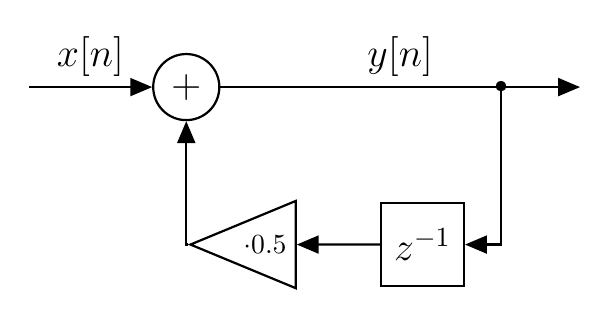
\begin{tikzpicture}[auto, thick, node distance=2.3cm, >=triangle 45]

  \draw node at (0,0) [input] (excitation) {};
  \draw node [sum, right of=excitation, node distance = 2.cm] (sum1) {\Large$+$};
  \draw node at (5,-2) [block ] (delay) {\Large$z^{-1}$};
  \draw node [mult,shape border rotate=180, left of=delay, node distance = 2cm] (loss) {$\cdot 0.5$};
  \draw node at (6.,-0.001) {\textbullet};

  \draw node [output, right of=sum1,node distance = 5cm] (out) {};
  \draw[->] (excitation) -- node {\Large$x[n]$}(sum1);
  % \draw[->] (sum1) -- node {}(6., -0.001);
  \draw[->] (loss.west) -| node {}(sum1.south);

  \draw[->] (6., -0.001) |- node {}(delay.east);
  \draw[->] (delay) -- node {}(loss);


  \draw[->] (sum1) -- node {\Large$y[n]$}(out);

  \end{tikzpicture}
  \caption{A simple IIR filter. Note that the arrows are circling, there is feedback involved.}
\end{figure}


If we look at the impulse Response, we can see that it is  ``longer'' than what we had before. If you look closely, we can see that the output sample at which the impulse arrives(n=3), just has the value of the input(1). After that, we can see that the next value is always the sample before times 0.5, so the impulse respopnse is a \textit{geometric series}: $\{1,0.5,0.25,0.125,..\}$ or $\{1, \frac{1}{2}, \frac{1}{4}, \frac{1}{8}, ...\}$. This is the case since the coefficient in the feedback path is 0.5, so $\frac{1}{2}$.


\begin{figure}[H]
	\centering
	\includegraphics[width=\textwidth]{IIR1}
	\caption[Impulse Response of $y(n)=x(n)+\frac{1}{2}y(n-1)$]
	{Impulse Response of $y(n)=x(n)+\frac{1}{2}y(n-1)$}
	\label{fig:label}
\end{figure}

Let's translate the above diagram to a difference equation, so we see another representation of the same system.
\begin{equation}
 	y(n) = x(n)+y(n-1) \cdot 0.5
 \end{equation}

Finally, let's quickly summarize some of the differences between the two filter types:
\begin{center}

\begin{tabular}{l|l|l}

& \textbf{IIR} & \textbf{FIR} \\
\hline
stability & possibly unstable & always stable \\
Real time Efficiency & Very efficient & inefficient \\
topology & Feedback & no feedback \\

\end{tabular}
\end{center}

% \section{Convolution}
% Convolution is a very important concept in DSP. We already encountered it in chapter \ref{Modulation}. We know that convolution reverbs use impulse responses of rooms to simulate these rooms. But how is this done? It \textit{can} be done using a FIR filter.




\section{Key Points}
\begin{itemize}
	\item Make sure you understood the differences between a FIR and an IIR filter.
	\item Make sure you can make an educated guess what kind of a filter we see if you encounter a block diagram.
	\item Make sure you can do simple translations between pd, blockdiagrams and difference equations.
	\item Make sure you know when a combfilter turns into a lowpass.
	\item Make sure you know and understand the formula to calculate the first phase cancellation in a combfilter.
\end{itemize}

\section{Homework}

Build the structure depicted in Figure~\ref{fig:genFx} in pd.

\begin{figure}[H]
	\centering
	\includegraphics[width=\textwidth]{img/effect.png}
	\caption[Generalized Effects Structure proposed by Dattoro]
	{Effects Structure proposed by Dattoro}
	\label{fig:genFx}
\end{figure}


% Notizen aus erster UE:\\
% Viellt. mit IR anfangen?
% Vielleicht davor noch: das beispiel mit noise + sinus.

% IR, bypass system, hall system.

% garnicht faltung. Moving average zu long FIR.
% Impuls antworten anhand beispielen besprechen.


% \begin{enumerate}
% 	\item FIR!

% kammfilter(FF)

% dann FIR kammfilter

% chorus
% flanger

% LFO

% ->index/tiefe, offset, frequenz wdh.


% -frequenzgang
% ausl\"oschungen, rechnen..

% \item
% FIR one sample delay\\

% FIR bauen, vllt. an tafel blockdiagramm.\\

% FIR hipass\\


% \item

% mehrere Samples delay
% IR
% differenzen gleichung

% eventuell Faltung(faltungs hall connection herstellen)

% faltung als multiplikation d. spektra
% multiplikation als faltung d spektra.

% M4L faltungs hall herzeigen

% LTI?

% differentiator, akkumulator?

% \item
% IIR\\



% notizen POlyphonie
% was separat, was einmal

% \end{enumerate}

% \section{einfuehrung} % (fold)
% \label{sub:einfuehrung}


% Ziel der LV:\\
% \begin{enumerate}
% 	\item Gefühl dafür bekommen was die häufigsten Operationen der DSV eigentlich tun.
% 	\item Gefühl dafür bekommen, dass es günstig ist, zwischen verschiedenen repräsentationen hin und her zu wechseln (time und frequency domain, aber auch system repräsentationen)
% 	\item Sich in professioneller literatur(DSP lehrbücher) nicht völlig verloren fühlen.
% 	\item schönheit zu sehen dass alles das \glqq{}gleiche\grqq{} ist.(Delay, filter, reverb, chorus, flanger etc)
% \end{enumerate}

% Wozu?:\\
% \begin{enumerate}
% 	\item Wir arbeiten ständig mit Operationen der DSV. Filter sind nicht nur in synthesizern. Ein tieferes verständnis erleichtert die arbeit. Wie funktioniert zum beispiel ein blur?
% 	\item Was ist ein FeedForward compressor?
% \end{enumerate}


% Nachdenken über filter allgemein. Was ist ein filter im gespür d. studenten. \\
% Bekannt was ein LTI system ist?\\


% \newpage
% -Wie könnte ein filter realisiert werden?\\
% -Ein digitales signal ist eine reihe von zahlen, eine sequenz von werten. (über bildliche darstellungen sprechen)\\
% -Echtzeit fall: ich bekomme in ein system ein signal(also ständig werte) und soll ein zb. lowpass gefilteretes signal ausgeben.\\
% \textbf{Was kann ich mit dem signal machen? Zum beispiel addieren, multiplizieren, verzögern.}\\


% Einfacher moving average. Zunächst nur an der tafel!
% Impulsantowrt ausrechnen!
% Was ist ein impuls.\\
% Was ist eine impulsantwort? Beispiele.. untit impulse ( = dirac impuls, dirac gunktion, delta function)\\

% Diagramm aufmalen:

% impuls \(\rightarrow\) Raum \(\rightarrow\) Impulsantwort\\
% oderr \\
% impuls \(\rightarrow\) beliebiges system \(\rightarrow\) Impulsantwort\\
% \textbf{anwendugsbeispiel:} tontechnik bei okto; mischpult ausmessen, dbmax ausmessen(fragwürdige sache! Wieso?)




% \textbf{FRAGE}\\
% Ein system(zB. ein Filter) hat folgende Eigenschft:\\
% Wenn zwei signale getrennt (d.h. unabhängig voneinander, zB. nacheinander.) in das system geschickt werden, und die Ergebnisse summiert werden, entsteht das signal \(P\). Wenn andererseits die signale zuvor summiert werden und dann in das system geschickt werden entsteht ebenfalls \(P\). Welche gleichung etspricht einer beschreibung dieser eigenschaft?



% \begin{enumerate}
% 	\item \(f(x)+f(y) = f (x * y) = P\)
% 	\item \(f(x)+f(y) = f (x + y) = P\)
% 	\item \(f(x)+f(x) = f (x + y) = P\)
% 	\item \(f(x)+f(y) = f (x + x) = P\)
% 	\item nichts von alledem.
% \end{enumerate}

% \newpage
% richtig : nr.2 \\
% \\

% Erklärung eines LTI systems:

% \begin{itemize}
% 	\item Linear:
% 		\begin{itemize}
% 			\item Superpositionsprinzip \(f(x)+f(y) = f (x + y)\)
% 			\item Homogenität \(a*f(x) = f(a*x)\)
% 		\end{itemize}
% 	\item Time Invariant (zeit-invariant)
% \end{itemize}


% Zurück zu filter:
% was glauben sie wie er funktioniert. \\
% \\

% \section {kammfilter}

% Wiederum fragen was sich die studenten vorstellen.\\


% \glqq{}Wir bauen ein delay.\grqq{}
% nicht vergessen: block~, subpatcher.


% \begin{figure}[h]
% 	\begin{center}
% 		\includegraphics[width = 14cm]{simpleDelay.png}
% 		\caption{SimpleDelay}
% 		\label{fig:simpleDelay}
% 	\end{center}
% \end{figure}

% Studenten sollen ausprobieren. Verschiedene inputs f. kammfilter. \\

% Modulation des kammfilters. Studenten sollen LFO an den kammfilter dran bauen.\\
% \(\rightarrow\) Flager \\
% \(\rightarrow\) Chorus \\

% \textbf{index/tiefe, offset, frequenz wiederholen.}


% \begin{figure}[h]
% 	\begin{center}
% 		\includegraphics[width = 14cm]{generalizedEffect.png}
% 		\caption{generalized Effect structure}
% 		\label{fig:genEffect}
% 	\end{center}
% \end{figure}

% über name sprechen, sowohl spectrum als auch Impulsantwort(IIR variante) sind kammförmig. \\
% Eigentlich einfach ein delay, ein delay mit feedback im falle von IIR.\\




% \begin{figure}[h]
% 	\begin{center}
% 		\includegraphics[width = 14cm]{img/combFIR_patch.png}
% 		\caption{Der Patch 01\_combFilter.pd}
% 		\label{fig:01_combFilter}
% 	\end{center}
% \end{figure}



% Zunächst nicht wichtig die versch. representationen zu verstehen. \\
% Patch representation kurz durchbesprechen. Sollte verständlich sein.\\

% Unterschiedliche representationen durchbesprechen.
% Fragen, abstimmen?, was die studenten für die angenehmste representation halten.



% \begin{itemize}
% 	\item Patch: vorteile: interaktiv, allgemein, reinfolge der events nachvollziehbar. Nachteil: nicht sehr übersichtlich. Nicht sehr konzis, nicht kompakt.
% 	\item Block Diagramm: übersichtlich, allgemein. Reinfolge der events klar, pfeile! Fluss, richtung, eindeutig. Nachteile: Nicht kompakt.
% 	\item differenzen gleichung: Vorteil: kompakt, konzis. Nachteil: reinfolge der events nicht klar ersichtlich: kein rezept, eher eine beschreibung. (nicht imperativ sondern deklarativ, va. im Fall von Feedback)
% 	\item Impulsantwort: \textbf{Frage: was ist ein Impuls?}  Vor/Nachteil: Nicht allgemein, nur ein spezieller zustand des systems beschrieben. Nicht kompakt, aber kann sehr intuitiv sein. Beispiele an tafel: IR von bypass-system, IR mit viel hall, IR von bandpass filter mit hoher resonanz, eventuell: differentiator, accumulator.
% 	\item andere representationen: text-code, transfer funktion, frequency response(magnitude + phase response/group delay)
% \end{itemize}




% \newpage


% \section {Moving Average}

% \textbf{Wo hat der kammfilter immer sein erstes Tal im spectrum?}
% Sinus an tafel malen.
% Antwort:
% bei

% \(\lambda =  (2* \Delta t) \)
% (wobei \(\Delta t\) die delay zweit in sekunden. und \(\lambda\)  die periodendauer der gesuchten frequenz.) Daher:\\
% \(
% f_c = 1/(2* \Delta t)
% \)

% Nun wird das delay auf ein sample reduziert. Ein lowpass entsteht der seine grenzfrequenz bei sr/2 hat.\\

% Frage: was macht ein lowpass filter in der timedomain?


% \begin{figure}[h]
% 	\begin{center}
% 		\includegraphics[width = 14cm]{movingAverage.png}
% 		\caption{movingAverage}
% 		\label{fig:movingAverage}
% 	\end{center}
% \end{figure}


% \textbf{EXKURS: VIDEO FILTER, lowpass, time domain erkennen.}


% \newpage
% \textbf{Frage:} Vergleiche original und die gefilterte variante (01.mov) . Was für ein filter könnte angewandt worden sein:
% \begin{enumerate}
%  	\item lowpass
%  	\item bandpass
%  	\item hipass
%  	\item notch
%  	\item nichts von alledem
%  \end{enumerate}


% wie könnte ein highpass realisiert werden? Wie schaut der effekt eines highpass filters in der frequenz- und wie in der timedomain aus?


% \section{convolution, Faltung}

% Video (unten) zeigen, vorher erklären: \\

% conv theorem.

% http://youtu.be/\_vyke3vF4Nk?t=25m16s \\
% start bei min 25.

% \textbf{maxpatch}




% %%--------------------------------------------------------------------------
% %% IIR/FIR
% %%--------------------------------------------------------------------------
% \section {IIR/FIR}

% Je steiler die Filterflanke sein, je komplexer der filter sein soll, desto mehr delays werden benötigt.\\

% Wieso: einfache Erklärung: Um aus einem signal, das alle frequenzen enthält (zB dirac impuls) ein signal zu machen, das hauptsächlich sehr tiefe frequenzen enthält wird ein system benötigt das \glqq{}lange wellen\grqq{} zu produzieren im stande ist.

% An tafel zeichnen: dirac impuls und unit step/ DC. Frage nach spectrum.\\

% frage nach FIR der diesen IR haben könnte.

% \textbf{Patch: lomgSimpleFir}

% Grenzfall: integrator macht aus unit impulse, \(delta [n]\), unit step signal\(u[n]\)(DC).

% Integrator an tafel malen.\\

% Daher:
% Es kann gezeigt werden dass ein feedback pfad einer unendlichen menge an delays gleichkommt, siehe IR.

% \textbf{Patch: 02\_combFilterIIR}

% nebenbei:
% linear phase = symmetrischer IR, immer FIR, daher weniger performant.
% Linear phase filter sind notwendig wenn die timedomain wellenform möglichst unbeeinträchtigt bleiben soll.

% \subsection{Onepole} % (fold)
% \label{ssub:onepole}

% % subsubsection subsubsection_name (end)
% onepole an tafel beschreiben. Block diagramm, malen, nach differenzengleichung fragen. Patch herzeigen.\\

% \textbf{patch: IIRtest} \\
% danach:\\
% \textbf{patch: IIRtest2} \\

% Fragwürdig aber falls interesse:
% onepole coeff berechnung zB:\\

% \begin{equation}
% a_0 = \frac{2 \pi f_c} {sr}
% \end{equation}

% oder

% \begin{equation}
% a_0 = sin(\frac{2 \pi f_c} {sr})
% \end{equation}


% \section{Hausübung}

% hausübung: Baue einen einen chorus. TESTSIGNAL AUSBESSERN! nicht noise!!

%!TEX root = main.tex
\chapter{Physical Modeling}
\label{Karplus}

\begin{figure}[h]
  \begin{center}
    \includegraphics[width = 14cm]{img/strohgeige.jpg}
    \caption{Die Strohgeige, ein eigentuemliches Saiteninstrument}
    \label{fig:metering}
  \end{center}
\end{figure}


\section{References}

\begin{itemize}
  \item \cite{bilbao_numerical_2009}
  \item \cite{smith_physical_2010}
  \item \cite{cook_real_2002}
\end{itemize}


% Karplus strong und PM,\\
% schwingungssysteme,\\
% simulation..

% Ableton Live: donner,\\
% rechtfertigung: Computerspiele, etc.\\
% (Wellen-)Experiment.\\
% Geschichte: Bernoulli und D'Alembert\\
% Wellengleichung
% Karplus Strong (bauen, geschichte erzählen)
% (Pause)
% Waveguide, Scattering Junctions erwähnen undje nach interesse behandeln. Kelly und Lochbaum modell.
% Kaffeehäferl synthetisieren. (Praat, reson)



\section{Further Information}

\begin{itemize}
  \item \link{https://www.youtube.com/watch?v=Li6OEMCtQ9k}{Wave Equation}
  \item \link{https://www.youtube.com/watch?v=dUcNzPhZdwk}{Julius O. Smith about Physical Modeling in Stanford}
  \item \link{http://www.fon.hum.uva.nl/praat/}{Praat audio analysis}
\end{itemize}



\section{Overview}


\begin{enumerate}
	\item motivation: games, and efficient realistic sound generation
	\item PM: erklärung
	\item Karplus-Strong
	\item Schulübung: sounddesign challenge in pd.

\end{enumerate}

\section{Theory: Oscillating Systems}


Wave equation, infinite one-dimensional string:
\begin{equation}
	c^2 \cdot \frac{\delta^2 f}{\delta x^2} = \frac{\delta ^2 f}{\delta t ^2}
\end{equation}

Visualization:

\begin{figure}[H]
  \begin{center}
    \includegraphics[width = 14cm]{img/wellengleichungVis.png}
    \caption{Visualisierung der Wellengleichung}
    \label{fig:wellengleichung}
  \end{center}
\end{figure}




Two possible solutions for the differential equation:
\begin{itemize}
	\item Bernoulli = ca. fourier, spectral, summe von sinus schwingungen.
	\item D'Alembert = ca. Physical modeling, zwei funktionen die entlang der saite reisen (in entgegengesetzte richtung).
\end{itemize}

Bernoulli:
\begin{equation}
  y(t,x) = \sum^{\infty}_{k=0} A_k sin(k\pi x/L)cos(k\pi \nu t)
\end{equation}
(Displacement length $L$, vibrating string at time $t$ at position $x$, frequency $\nu$)

\begin{equation}
y(x, t) = y ^+ \Bigg(t - \frac{x}{c}\Bigg) + y^- \Bigg(t + \frac{x}{c} \Bigg)
\end{equation}

\section{Karplus Strong Synthesis}
% D'Alembert sagt also, es gäbe zwei wellen, die in zwei richtungen entlang der saite reisen, die Lässt sich einfach simulieren, mittels zwei in einander geschalteten delays.
So D'Alembert says, there are two waves, one traveling to the right and one traveling to the left. Their superposition is what makes up the actual wave along a string. \\
Observing a string more closely, we find that a wave gets inverted at its borders and travels back.
All this can easily be simulated in a computer, see Figure~\ref{fig:string}.


  \begin{figure}[htb]
  \centering
  \label{fig:string}

  % \resizebox{10cm}{!}{%
  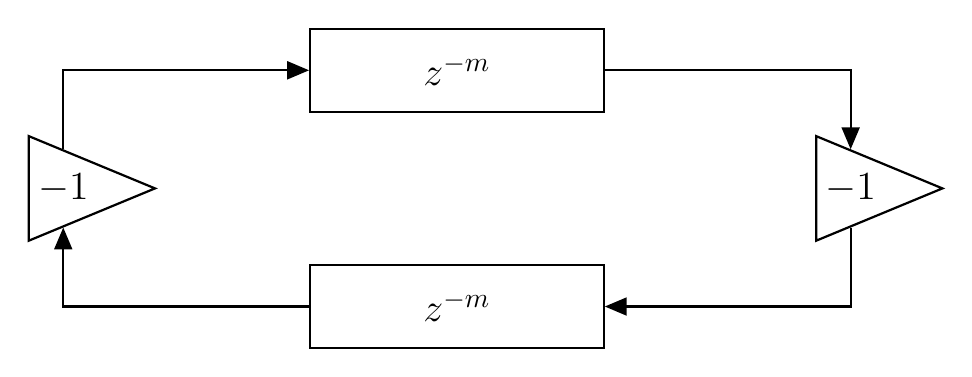
\begin{tikzpicture}[auto, thick, node distance=2.3cm, >=triangle 45]

  \draw node at (5,0) [block] (del1) {\Large$\ \ \ \ \ \ \ \ z^{-m}\ \ \ \ \ \ \ \ $};
  \draw node at (5,-3) [block] (del2) {\Large$\ \ \ \ \ \ \ \ z^{-m}\ \ \ \ \ \ \ \ $};
  \draw node at (0, -1.5) [mult] (m1) {\Large$-1$};
  \draw node at (10, -1.5) [mult] (m2) {\Large$-1$};

  \draw[->] (del1) -| node {}(m2);
  \draw[->] (m2) |- node {}(del2);
  \draw[->] (del2) -| node {}(m1);
  \draw[->] (m1) |- node {}(del1);

  \end{tikzpicture}
  \caption{general idea of Waveguide synthesis/Karplus-Strong Model.}
\end{figure}

The model in Figure~\ref{fig:string} is a rather theoretical one\footnote{You might notice that there are no inputs and no outputs. This structure is theoretical for us, since we do not talk about something called the \textit{Wave Digital Filter}(WDF). When talking about WDFs we find similar structures since they are strongly inspired by physics. Since in physics we always have a force and another force counteracting the first one we always have left and right traveling energy.}. But it leads us to a more useful implementation. Since all elements in Figure~\ref{fig:string} are LTI, we can rearrange them in any order. Multiplying a signal times $-1$ two times is the same as doing nothing. And two delays of length $m$ are equivalent to one delay of length $2m$.\\
So we arrive at a simple delay with feedback. To simulate energy loss we need to attenuate the feedback signal and to simulate frequency dependent loss, we can use a lowpass filter inside the feedback loop. After all this, we arrive at Figure~\ref{fig:string2}.

\begin{figure}[h!]
  \centering

  \label{fig:string2}

  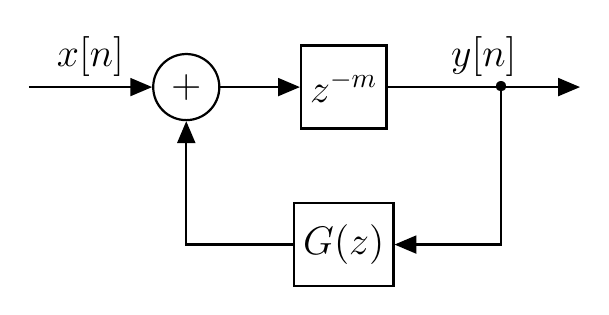
\begin{tikzpicture}[auto, thick, node distance=2.3cm, >=triangle 45]

  \draw node at (0,0) [input] (excitation) {};
  \draw node [sum, right of=excitation, node distance = 2.cm] (sum1) {\Large$+$};
  \draw node [block, right of=sum1, node distance = 2cm] (delay) {\Large$z^{-m}$};
  \draw node [block, below of=delay, node distance = 2cm] (loss) {\Large$G(z)$};
  \draw node at (6.,-0.001) {\textbullet};

  \draw node [output, right of=delay,node distance = 3cm] (out) {};
  \draw[->] (excitation) -- node {\Large$x[n]$}(sum1);
  \draw[->] (sum1) -- node {}(delay);
  \draw[->] (loss.west) -| node {}(sum1.south);

  \draw[->] (6., -0.001) |- node {}(loss.east);


  \draw[->] (delay) -- node {\Large$y[n]$}(out);

  \end{tikzpicture}
  \caption{single string, $G(z)$ a lowpass, \glqq{}Loss Filter\grqq{}}
\end{figure}

\section{Practical Karplus-Strong}
\begin{figure}[H]
	\begin{center}
		\includegraphics[scale = 1.]{img/karplusSimple.png}
		\caption{Basic setup, a delay with feedback.}
		\label{fig:karplusBasic}
	\end{center}
\end{figure}


\begin{figure}[H]
  \begin{center}
    \includegraphics[scale = 0.3]{img/karplusComplete.png}
    \caption{Complete Algorithm}
    \label{fig:karplusComplete}
  \end{center}
\end{figure}



\section{Modal Synthesis with Bandpass filters}


\section{Schulübung, Sounddesign challenge}

zB:
\begin{itemize}
	\item Vokal
	\item E-gitarre
	\item beliebiges Physikalisches object

\end{itemize}

\section{Key Points}
\begin{itemize}
  \item Make sure you understood how the Karplus-Strong algorithm works and know its structure.
  \item Make sure you understand what the elements of the karplus strong algorithm might mean (physical analogies).
\end{itemize}


% \section{Hausuebung}
% Andy Farnell, \href{http://aspress.co.uk/ds/pdf/pd_intro.pdf}{pd intro} chater 7, lesen


%!TEX root = main.tex

\chapter{Fourier Transform}
\label{Fourier Transformation}

\begin{figure}[H]
	\begin{center}
		\includegraphics[width = 14cm]{img/aphexFFT.png}
		\caption{Image in the spectrogram in a track by ``Aphex Twin''.}
		\label{fig:Aphex}
	\end{center}
\end{figure}




\begin{center}
\begin{figure}[H]
\tikzset{concept/.append style={fill={none}}}
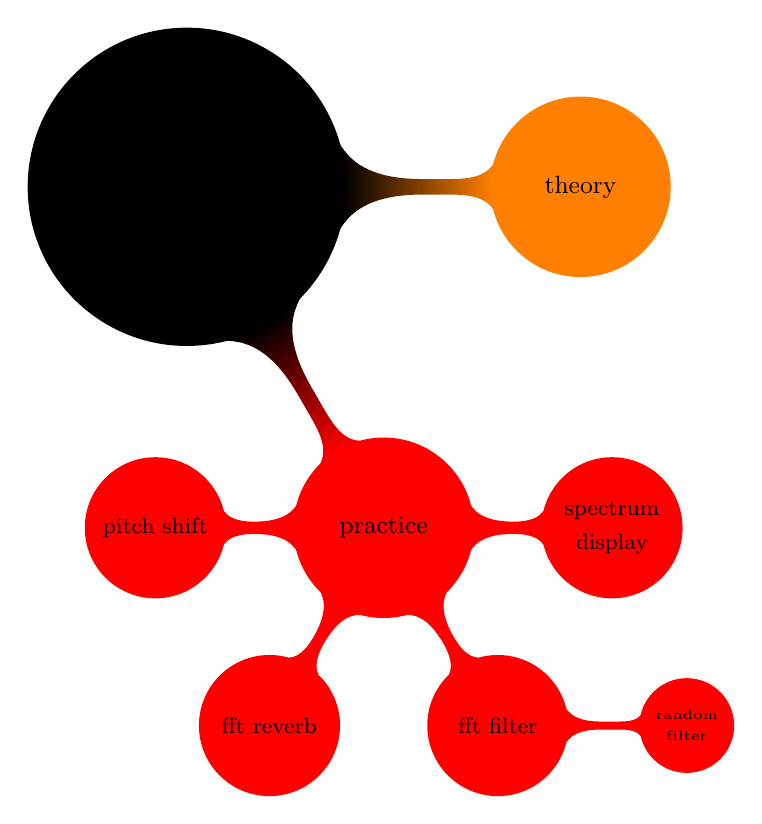
\begin{tikzpicture}
  \path[mindmap,concept color=black,text=black]
	node[concept] {Fourier Tansform}
	[clockwise from=0]
	% child[concept color=green!50!black] {
	% node[concept] {schuluebung v. letzem Mal}
	% }
	% child[concept color=green!50!black] {node[concept] {pd parxis}
	% 	child[concept color=green!50!black] {node[concept] {send/receive}}
	% 	child[concept color=green!50!black] {node[concept] {initialisierung}}
	% 	}
	% child[concept color=blue] {
	% node[concept] {hauptteil FFT}
	% [clockwise from=-90]
		child[concept color=orange] { node[concept] {theory} }
		child[concept color=red] { node[concept] {practice}
			child[concept color=red] { node[concept] {spectrum display} }
			child[concept color=red] { node[concept] {fft filter}
				child[concept color=red] { node[concept] {random filter} }
				}
			child[concept color=red] { node[concept] {fft reverb} }
			child[concept color=red] { node[concept] {pitch shift} }
		}


;
\end{tikzpicture}
\caption{Lecture Contents: Fourier Transform}
\end{figure}
\end{center}

\section{Further Information}

\begin{itemize}
	\item \link{https://www.youtube.com/watch?v=-IJuqR6nz\_Q}{complex Numbers}
	\item \link{https://www.youtube.com/watch?v=EIstpPXKWng}{The Imaginary Number}
	\item \link{http://jackschaedler.github.io/circles-sines-signals}{Interactive Visualization of the Fourier Transform}

\end{itemize}

% vorbereitung:\\
% Eulers identity, complex numbers.



% Initialisierung
% Fourier transformation.
% Spectral filter
% Spectral Reverb, delay.
% Windowing
% Convolution,
% evtl. cross correlation
% freq. crossover
% spectral synyth,
% spectraum display.


% evtl auch:
% \begin{itemize}
% 	\item send / receive, send / receive bei gui objekten.
% 	\item initialisierung
% 	\item
% \end{itemize}


% Diskretes Signal -> Periodisches Spectrum \\
% Periodisches Signal -> Diskretes Spectrum



% fftuebung
% beiwerk:
	% initialisierung
	% send/receive
% schuluebung von letzem mal
% hauttteil fft
	% theorie	> geschichte
	% praxis
		% spectrum display
		% fft filter
			% nomral
			% random
		% fftdelay
		% fft reverb
		% pitch shift


% \section{Fourier Transformation}
\section{Concept}
The Fourier transform is a way to switch domains. What does that mean? We can think of it as transforming a piece of information into another representation without loss of information. To give an analogy: \\
If I tell you, we meet at \textit{Matthias Corvinus-Straße 15, 3100 St. Pölten} it is the same as telling you we meet at GPS coordinates 48.2138731, 15.6320195. It is the same information in another format, another \textit{domain}.\\
These two formats have different advantages and disadvantages. For example, would you know if the location in GSP format is even in Austria? Probably not. On the other hand, in which direction (north, south, east, west) do I have to go from the FH to get to the main train station? easy to see GPS: the main train station is at 48.20850,15.62515. Both numbers are lower so it must be south west. Not so easy to see if I tell you the train station is at Bahnhofplatz 1,3100 St. Pölten. \\
The point is, depending on what we want, different representations offer different possibilities and insights.
\begin{figure}[H]
	\centering
	\includegraphics[width=\textwidth]{img/vase.jpg}
	\caption[illusion]
	{Depending on how you look at something, different possibilities and insights arise.}
	\label{fig:vase}
\end{figure}

In the case of the Fourier transform we want to switch to a spectral domain. We want to do this since it would enable us to immediately see if there is a lot of energy at a certain frequency. Oddly, with light in the physical world, this seems very simple, just take a prism:

\begin{figure}[H]
	\centering
	\includegraphics[width=\textwidth]{img/Prism.jpg}
	\caption[prism]
	{A prism splits up light into its different spectral components, essentially performing a Fourier transform.}
	\label{fig:prism}
\end{figure}

\section{Math}
So how do we do this domain switching? There are different approaches to explaining what's happening in the Fourier Transform, but I think this is the most intuitive one: Remember, we just want to know how much of a certain frequency is contained in a certain signal $x(t)$.\\
If I give you 100 Euros and ask you to tell me how many 5 Euro bills are "in there", what would you do? Divide, of course. So can we just take a time domain signal and divide it by a sine at some frequency to see how much of it is contained in that signal? Yes!\\
The Fourier transform is defined as

\begin{equation}
	X(f)= \mathcal{F} \{x(t)\} = \int_{-\infty}^\infty \! x(t) e^{-i2\pi ft} \, \mathrm{d}t
	\label{ft}
\end{equation}

Most of the time we are dealing with discrete (digital) signals, but since the  \textit{Discrete Fourier Transform} (DFT) is a bit less intuitive, let's stick to the continuous('analog') one.


What does Equation \ref{ft} mean? We have an input time domain signal $x(t)$. We get out a frequency domain signal $X(f)$. In order to see why this is working, we need to remember Euler's identity:

\begin{equation}
	e ^{ix} = cos(x)+i \cdot sin(x)
\end{equation}

So, the Fourier transform actually is an integral (a continuous summation) over the input signal times cosine and sine terms:


\begin{equation}
	X(f)= \mathcal{F} \{x(t)\} = \int_{-\infty}^\infty \! x(t) \cdot (cos(2\pi ft)+i \cdot sin(2\pi ft) )^{-1}  \, \mathrm{d}t
	\label{ft2}
\end{equation}

And, knowing that a negative exponent means the same as using the reciprocal, so dividing, we can rearrange to:


\begin{equation}
	X(f)= \mathcal{F} \{x(t)\} = \int_{-\infty}^\infty \! \frac{x(t)} { cos(2\pi ft)+i \cdot sin(2\pi ft) }  \, \mathrm{d}t
	\label{ft2}
\end{equation}

Now you can probably see that we just take the input signal, and for each frequency $f$, we just "sum" over the whole input signal to see how much sine and cosine of that frequency is contained. Ok, it's complex sinusoids, we didn't touch on complex numbers etc, but this should give you a feeling why this can work.

% \begin{equation}
% 	x_f(m) = \sum_{n=0}^{N-1} x(n)\cdot (cos(2 \pi \frac{n m}{N})+i \cdot sin(2 \pi \frac{n m}{N}))^{-1}
% \end{equation}


For the sake of completeness, here are some variants of the whole scheme:\\
% Geschichte:
% Bernoulli, Euler, Gauß, Fourier
The discrete Fourier Transform (DFT) is defined as:
\begin{equation}
	x_f(m) = \sum_{n=0}^{N-1} x(n)\cdot e^{-i 2 \pi \frac{n m}{N} }
	\label{eq:dft}
\end{equation}


Inverse Fourier Transformation:\\
\begin{equation}
	x(t)= \mathcal{F}^{-1} \{X(f)\} = \int_{-\infty}^\infty \! X(f) e^{j2\pi ft} \, \mathrm{d}f
\end{equation}

\section{Implementation}


As python code this could look like the following. Please refer to Equation \ref{eq:dft}. The code below uses the same variable names to make this as little confusing as possible.
\newpage
\lstinputlisting[language=Python,caption={DFT in python},captionpos=b]{code/fourierTransform.py}
The above code produces the following plot:
\begin{figure}[H]
	\centering
	\includegraphics[width=\textwidth]{img/pythonDFT.png}
	\caption[DFT Plot]
	{Plot produced by the script above.}
	\label{fig:pyfft}
\end{figure}

% \comm{Note: X axis in fig \ref{fig:pyfft} is wrong! Should go from 0 to 22050 and back to 0.}

Beware that the python code above implements Equation \ref{eq:dft} directly. It is \textit{very} slow. Typically, a different algorithm is used, such as an implementation of the Fast Fourier Transform (FFT). In python, there are several ways to compute an FFT in an efficient way such as \texttt{numpy.fft.fft()}. The FFT is a classic \textit{divide and conquer} solution to performance boosting an algorithm.\\
We need to address something here: We send a single frequency into the DFT and we expect a single spike, showing that we have energy at one frequency. And we get two peaks. This is because the FFT produces a mirrored, a two-sided spectrum. Basically, \textbf{you can ignore half of the plot}. Why is that? The explanation has to do with the fact that digital signals always have an infinite periodic spectrum. You might connect this to the phenomenon of aliasing.

\video{
	In video and image processing, the DFT does not play such a big role as in audio, but the discrete cosine transform does. The differences between the DFT and the DCT are:
	\begin{itemize}
		\item The DCT produces a real output, the DFT a complex one
		% \item The DCT has more resolution in the low-Frequency range
		\item there are several different forms of DCT and there is also the discrete Sine Transform (DST)
		\item The DCT tends to have more energy in its low frequency bins and is therefore more suitable for lossy data-compression (since we throw away high frequency or low energy bins)
	\end{itemize}
	For more information on the DCT and compression have a look at \href{https://www.youtube.com/watch?v=Q2aEzeMDHMA}{Jpeg compression and the discrete Cosine Transform}\footnotemark
}
\footnotetext{https://www.youtube.com/watch?v=Q2aEzeMDHMA}
\section{Application in pd}
We won't code a DFT in pd. Probably it's possible but didactically it wouldn't be very helpful and practically it would be a pita\footnote{Certain kind of bread.}. But we need to know how to use the FFT in pd. There are 4 objects of particular interest here:
\begin{itemize}
	\item \pd{fft\textasciitilde} fast (discrete) fourier transform
	\item \pd{ifft\textasciitilde} fast (discrete) inverse fourier transform
	\item \pd{rfft\textasciitilde} fast (discrete) fourier transform, real only
	\item \pd{rifft\textasciitilde} fast (discrete) inverse fourier transform, real only
\end{itemize}
The 'real only' versions assume that our time domain signals are not complex, so have no imaginary component, which is almost always the case.
\subsection{Filtering using the FFT}
\begin{figure}[h]
	\begin{center}
		\includegraphics[width = 14cm]{img/spectralFilter2.png}
		\caption{patcher: \texttt{patchers/05\_fourier/fftFilter.pd}}
		\label{fig:spectralFilter}
	\end{center}
\end{figure}
\subsection{Displaying the spectrum}
\begin{figure}[h]
	\begin{center}
		\includegraphics[width = 14cm]{img/showspectrum.png}
		\caption{showspectrum}
		\label{fig:showspectrum}
	\end{center}
\end{figure}

\section{Key Points}
\begin{itemize}
	\item Make sure you understood the formula for the Fourier Transform.
	\item Make sure you understand the (complex) output of a Fourier Transform and how to convert to amplitude and phase.
	\item Make sure you know Euler's formula by heart.
\end{itemize}


% \include{polyPhony}

% ---------SEMESTER4----------
\part{Semester 4} % (fold)
\label{prt:semester4}

%!TEX root = main.tex
\chapter{Jitter}
\label{Jitter}
\section{Notizen}

\section{Überblick}
\begin{itemize}
	\item Stundenwiederholung
	\item Überblick über Software Pakete
	\item Vizzie
	\item kommunikation pd/max?
	\item Aufgabe: Video Laden, Abspielen, Audio analyse, modulation eines Effektes, Recording.
	\item Jitter Matrix (Wiederholung?)
	\item Audio analogien: jit.convolve, anti-aliasing(Open GL), jit.charmap(lookup table)

	\item Open GL, anti aliasing,
\end{itemize}

\section{Andere Software Pakete für visuelle Echtzeit Arbeit}
Siehe \link{http://www.github.com/hrtlacek/rtv}{http://www.github.com/hrtlacek/rtv}

Graphik Programmierumgebungen
\begin{itemize}
	\item Jitter
	\item Gem (pure Data)
	\item vvvv
	\item TouchDesigner
	\item processing
	\item Quarz Composer
\end{itemize}
\glqq{}Professionelle\grqq{} weniger offene Systeme(weniger programmier-orientiert)
\begin{itemize}
	\item Watchout
	\item Vizrt
	\item Ventuz
\end{itemize}
Game Engines
\begin{itemize}
	\item Unreal 4
	\item Unity
	\item Cry Enigine
	\item ...
\end{itemize}


\section{Introduction}

\begin{figure}[h]
	\begin{center}
		\includegraphics[width = 14cm]{img/lookAtMatrix.png}
		\caption{How to look at a jitter matrix}
		\label{fig:howToLook}
	\end{center}
\end{figure}

\begin{figure}[h]
	\begin{center}
		\includegraphics[width = 14cm]{img/hiLevelJitter.png}
		\caption{hi Level Jitter}
		\label{fig:hiLevelJitter}
	\end{center}
\end{figure}

\begin{figure}[h]
	\begin{center}
		\includegraphics[width = 14cm]{img/VizzieAudioModulated.png}
		\caption{VizzieAudioModulated}
		\label{fig:VizzieAudioModulated}
	\end{center}
\end{figure}

\begin{figure}[h]
	\begin{center}
		\includegraphics[width = 14cm]{img/basicGL.png}
		\caption{basicGL}
		\label{fig:basicGL}
	\end{center}
\end{figure}


\begin{figure}[h]
	\begin{center}
		\includegraphics[width = 14cm]{img/openGLAdvanced.png}
		\caption{openGLAdvanced}
		\label{fig:openGLAdvanced}
	\end{center}
\end{figure}


\begin{figure}[h]
	\begin{center}
		\includegraphics[width = 14cm]{img/specViz.png}
		\caption{specViz}
		\label{fig:specViz}
	\end{center}
\end{figure}





%Verzeichnis aller Bilder
\newpage
\listoffigures

\newpage
\lstlistoflistings

%Literaturverzeichnis
\newpage
% unsrtdin
\bibliographystyle{apalike}
\bibliography{eproLib}

\end{document}
